\section*{Learning Objectives}
\begin{itemize}
\item Learn how to define coordinates in a subspace of $\real^n$ and understand how many coordinates you need.
\item An introduction to eigenvalues and eigenvectors of square matrices.
\item Applying to matrices some of the essential concepts in Linear Algebra.
\end{itemize}

\section*{Outcomes}
\begin{itemize}
\item Basis vectors, dimension, and coordinates
\item Eigenvalues, eigenvectors, and understanding when when eigenvectors provide a basis of $\real^n$.
\item Range of a matrix and its relation to column span and null space.
\item Handy matrix properties dealing with rank and nullity.

\end{itemize}




\newpage



\begin{figure}[h]%
\centering
\subfloat[]{%
    \label{fig:R2naturalBasisVectorsa}%
	\centering
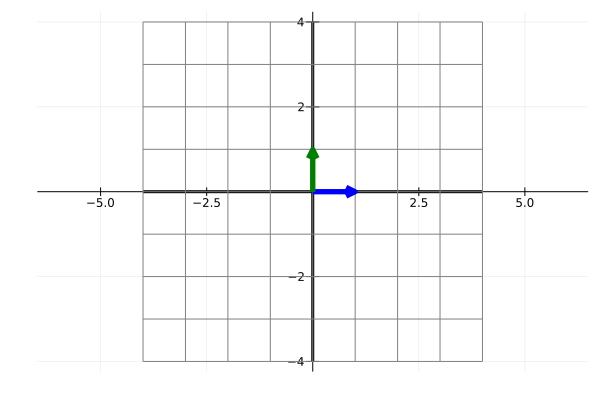
\includegraphics[width=0.45\columnwidth]{graphics/Chap10Rn/BasisUV01.png}}%
\hspace{5pt}%
\subfloat[]{%
    \label{fig:R2naturalBasisVectorsb}%
	\centering
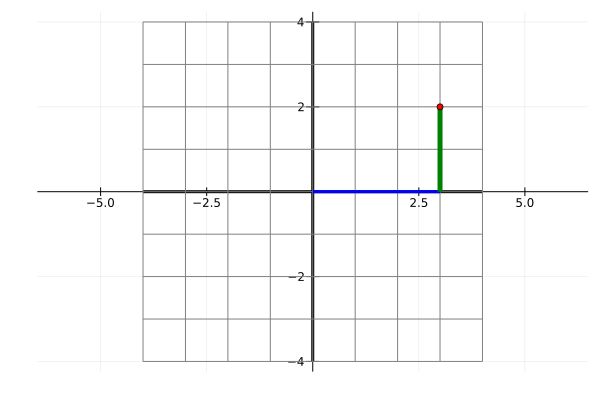
\includegraphics[width=0.45\columnwidth]{graphics/Chap10Rn/BasisUV01withpoint.png}}%
\hspace{5pt}%
    \subfloat[]{%
    \label{fig:R2Basisvectors01a}%
	\centering
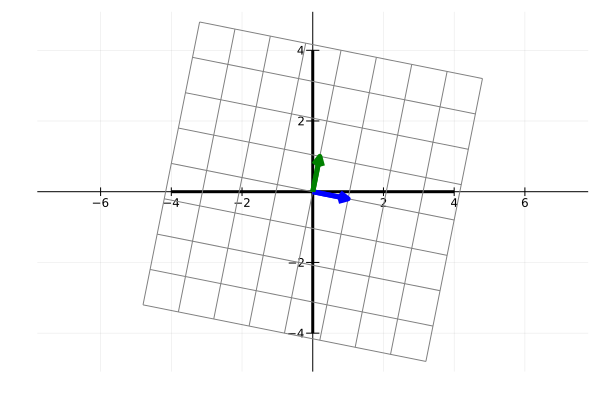
\includegraphics[width=0.45\columnwidth]{graphics/Chap10Rn/BasisUV02.png}}%
\hspace{5pt}%
\subfloat[]{%
    \label{fig:R2Basisvectors01b}%
	\centering
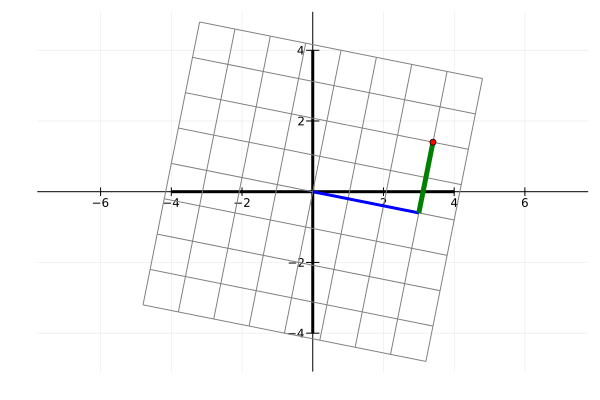
\includegraphics[width=0.45\columnwidth]{graphics/Chap10Rn/BasisUV02withpoint.png}}%
    \caption[]{Basis vectors $\{ \textcolor{blue}{u}, \textcolor{green}{v}\}$ (blue and green) for $\real^2$ with the corresponding coordinates. The graphs (a) and (b) show coordinates on $\real^2$ with the natural basis vectors, $\{u=e_1, v=e_2 \}$. The red dot in (b) is the point $3 u + 2 v$, that is, the point with coordinates $(3,2)$ in the basis $\{u, v \}.$  The graphs (c) and (d) show coordinates on $\real^2$ with basis vectors, $\{u=[1.0, -0.2 ]^\top, v= [0.2, 1.0]^\top \}$. The red dot in (b) is the point $3 u + 2 v$, that is, the point with coordinates $(3, 2)$ in the basis $\{u, v \}$. You go along the $u$-axis for three units and then follow the $v$-axis for two units. That is what the point $(3,2)$ means in a basis  $\{u, v \}.$ The vectors in the second basis are still orthogonal, because $ u \bullet v = 0$. They are rotated a few degrees clockwise with respect to the natural basis, however, and their lengths are not equal to one. When we study eigenvectors, you'll see a clear motivation for using bases on $\real^n$ that are distinct from the natural basis. For now, we are just saying that we can use different basis vectors, but not why we might want to do that.
    }
    \label{fig:R2BasisVectors}
\end{figure}


\section{Motivation}
Our first main topic, the notion of coordinates, links the notions of basis vectors, subspace, and dimension in a very tangible manner. 
 Eigenvalues and eigenvectors are required in EECS 442 (Computer Vision), EECS 445 (Machine learning), and ME 561 (Digital Control). The material on rank and nullity collects in one place useful facts that your author had to learn over his \textit{first five or six years} of using Linear Algebra. Having them all in one place like this is almost too nice of a gift! 


\section{Basis Vectors, Coordinates, and Dimension}
\label{sec:BasisCoordinatesDimension}


\begin{figure}[!hb]%
\centering
\subfloat[]{%
    \label{fig:R2naturalBasisVectorsA}%
	\centering
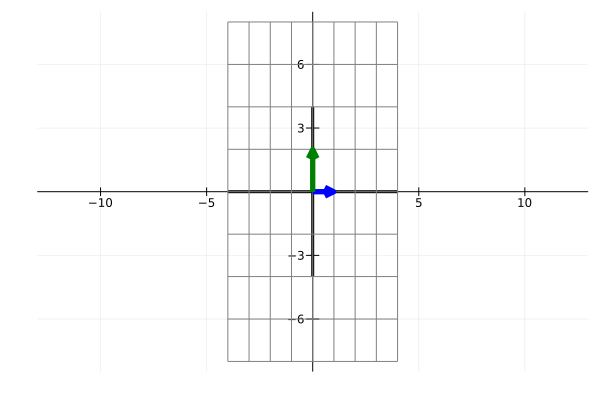
\includegraphics[width=0.40\columnwidth]{graphics/Chap10Rn/BasisUV03.png}}%
\hspace{5pt}%
\subfloat[]{%
    \label{fig:fig:R2naturalBasisVectorsB}%
	\centering
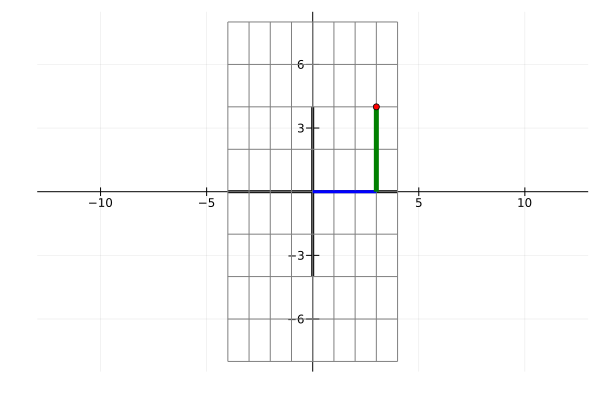
\includegraphics[width=0.40\columnwidth]{graphics/Chap10Rn/BasisUV03withpoint.png}}%
\hspace{5pt}%
    \subfloat[]{%
    \label{fig:R2BasisvectorsA}%
	\centering
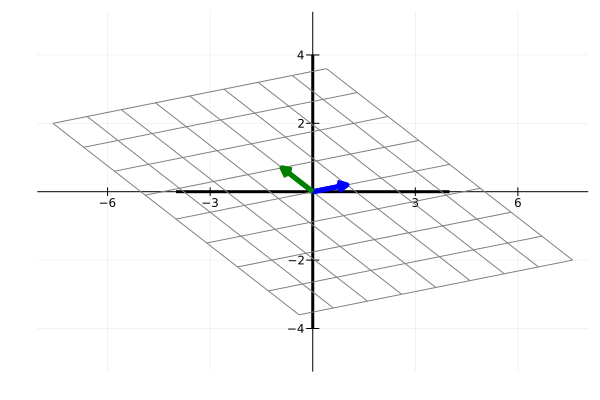
\includegraphics[width=0.40\columnwidth]{graphics/Chap10Rn/BasisUV04.png}}%
\hspace{5pt}%
\subfloat[]{%
    \label{fig:R2BasisvectorsB}%
	\centering
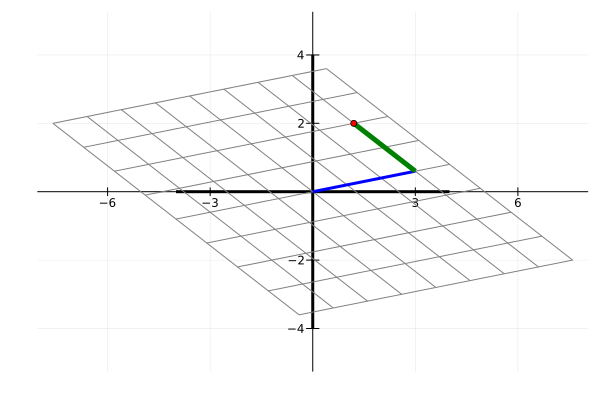
\includegraphics[width=0.40\columnwidth]{graphics/Chap10Rn/BasisUV04withpoint.png}}%
    \caption[]{Basis vectors $\{ \textcolor{blue}{\bf u}, \textcolor{green}{\bf v}\}$ (blue and green) for $\real^2$ with the corresponding coordinates. The graphs (a) and (b) show coordinates on $\real^2$ with the ``almost natural'' basis vectors, $\{u=e_1, v=2 e_2 \}$.  Note that we now have a rectangular grid instead of a square grid because the lengths of $u+e_1$ and $v=2 e_2$ are not equal. The red dot in (b) is the point $3 u + 2 v$, that is, the point $(3,2)$ in the basis $\{u, v \}.$  The graphs (c) and (d) this time show coordinates on $\real^2$ with basis vectors, $\{u=[1.0,  0.2 ]^\top, v= [-0.9, .7]^\top \}$, which are not orthogonal.  \textbf{Some of you may see the grid rotated out of the plane of the page...is so, this is an optical illusion. Everything is plotted in the same plane}. The red dot in (b) is still the point $3 u + 2 v$, that is, the point $(3, 2)$ in the basis $\{u, v \}$.  You go along the $u$-axis for three units and then follow the $v$-axis for two units.
    }
    \label{fig:R2BasisVectorsNotOrthognal}
\end{figure}


We consider $\real^n$ again, and define some special vectors. 
Let $I_n$ be the $n \times n$ identity matrix. Then $e_i:= i$-th column of $I_n$. For example, when $n=4$,
$$e_1 = \left[\begin{array}{c}  1 \\ 0 \\ 0 \\ 0\end{array} \right], 
e_2 = \left[\begin{array}{c}  0 \\ 1 \\ 0 \\0  \end{array} \right],
e_3 = \left[\begin{array}{c}  0 \\ 0 \\ 1 \\0  \end{array} \right],
e_4 = \left[\begin{array}{c}  0 \\ 0 \\ 0 \\1  \end{array} \right].$$

Looking at $\real^2$ just to make things definite, we recall that $\{e_1, e_2\}$ is a linearly independent set, because
\begin{equation}
\label{eq:R4ExampleBasis_a}
    \left( \alpha_1 e_1 + \alpha_2 e_2 =  \left[\begin{array}{c}  \alpha_1 \\ \alpha_2 \end{array} \right] = \left[\begin{array}{c}  0 \\ 0 \end{array} \right] \right) \iff \Big( \alpha_1=0, \alpha_2 = 0 \Big).
    \end{equation}
An important property of the set $\{e_1, e_2\} \subset \real^2$ is that any vector $x\in \real^2$ can be written as a linear combination of $e_1, e_2$. Indeed, 
\begin{equation}
\label{eq:R4ExampleBasis_b}
x=:\left[\begin{array}{c}  x_1 \\ x_2 \end{array} \right] = x_1 \left[\begin{array}{c}  1 \\ 0 \end{array} \right] + x_2 \left[\begin{array}{c}  0 \\ 1 \end{array} \right]= x_1 e_1 + x_2 e_2. 
    \end{equation}
Moreover, there is \textbf{only one linear combination} of  $\{e_1, e_2\}$ that yields the point $x = \left[x_1, x_2 \right]^\top \in \real^2$.







\begin{figure}[h]%
\centering
\subfloat[]{%
    \label{fig:Chap10Rn:CoordinatesA}%
	\centering
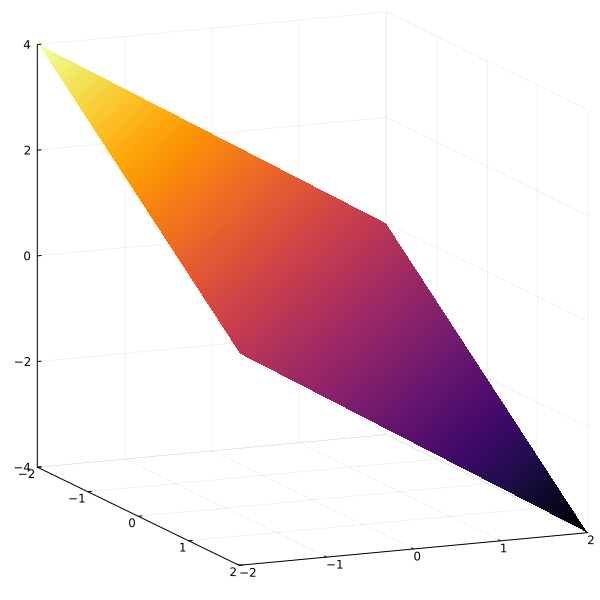
\includegraphics[width=0.3\columnwidth]{graphics/Chap10Rn/SurfaceInR3.png}}%
\hspace{5pt}%
\subfloat[]{%
    \label{fig:Chap10Rn:CoordinatessB}%
	\centering
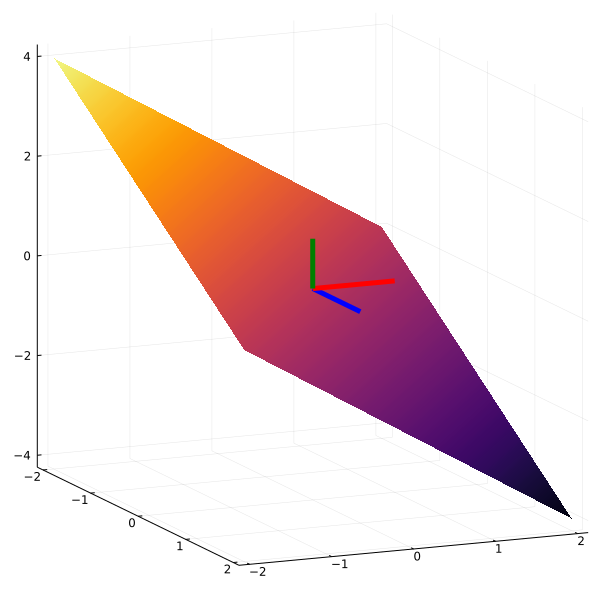
\includegraphics[width=0.3\columnwidth]{graphics/Chap10Rn/SurfaceInR3CanonicalBasisVectors.png}}%
\hspace{5pt}%
    \subfloat[]{%
    \label{fig:Chap10Rn:CoordinatesC}%
	\centering
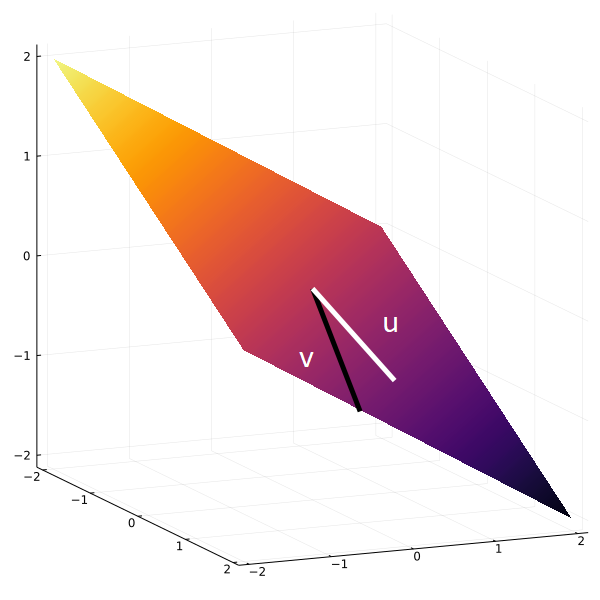
\includegraphics[width=0.3\columnwidth]{graphics/Chap10Rn/SurfaceInR3With2DBasisVectors.png}}%
    \caption[]{$\real^3$ with a two-dimensional subspace $z = -(x+y)/2$ (the colored planar surface) that we'll call $V$ in shown in (a), while part (b) shows the natural basis (which gives the $(x, y, x)$ coordinates in $\real^3$) do not lie in $V$ and hence do not form natural coordinates for the surface. \textbf{Hence, expressing locations in $V$ in terms of the ``natural coordinates'' $\mathbf{(x, y, x)}$ from $\real^3$ is not very natural at all!} It is much simpler, and more natural, to express points in $V$ in terms of basis vectors that lie in the plane, such as the vectors $\{ u, v\}$ shown in (c). Here, the vectors $\{ u, v\}$ were NOT selected to be \textit{orthogonal}, but we could have applied G-S and produced an orthonormal basis for $V$. Any pair of linearly independent vectors in $V$ will work, as illustrated in Figures~\ref{fig:R2BasisVectors} and \ref{fig:R2BasisVectorsNotOrthognal}.
    }
    \label{fig:Chap10Rn:CoordinatesNew}
\end{figure}


%\vspace*{.2cm}

\begin{tcolorbox}[sharp corners, colback=green!30, colframe=green!80!blue, title=\textbf{\Large Basis Vectors and Dimension}]
Suppose that $V$ is a subspace of $\real^n$. Then $\{ v_1, v_2, \ldots, v_k\}$ is a \textbf{basis for} ${\bf V}$ if
\begin{enumerate}
    \item the set $\{ v_1, v_2, \ldots, v_k\}$ is linearly independent, and 
    \item $\spanof{v_1,  v_2,\ldots, v_k}=V$.
\end{enumerate}

The \textbf{dimension of} ${\bf V}$ \textbf{is} ${\bf k}$, the number of basis vectors\footnote{A more correct definition is the maximum number of vectors in any linearly independent set contained in $V$. For ROB 101, the definition we gave is good enough}.\\

We note that the above definition applies to $\real^n$ \textbf{because} $\real^n$ is a subset of itself and it is closed under linear combinations. In particular, $\real^n$ has dimension $n$, or we say that $\real^n$ is an $n$-dimensional vector space.
\end{tcolorbox}

\begin{tcolorbox}[title=\textcolor{red}{\bf \Large Basis Intuition}]
The essence of a \textbf{basis}: a set of vectors that is (a) ``small enough'' to be linearly independent and yet (b) ``big enough'' to generate all vectors in a vector space or a subspace by forming linear combinations.\\

Yes, it's kind of a \textcolor{red}{\bf ``Goldilocks'' notion:} a set of vectors that is \textcolor{red}{\bf not too big} (linearly independent) and \textcolor{red}{\bf not too small} (spans the subspace). \textcolor{red}{\bf Just the right size! }\\

If we add one more vector to a basis for $V$, then either the new set will become linearly dependent or it will span a set that is larger than $V$. If we take away even one vector from a basis, then it will no longer span the original set. So yes, a basis really is a ``Goldilocks'' notion.
\end{tcolorbox}
\vspace*{.1cm}
Basis vectors are important because they provide a simple means to generate all vectors in a vector space or a subspace by forming linear combinations from a finite list of vectors. The basis and the subspace can be essentially treated as one and the same object when it comes to computations: we can manipulate a subspace in a computer by computing with its basis vectors! \textbf{An under appreciated aspect of a \textcolor{red}{basis}   for a subspace $V$ is that it  \textcolor{red}{defines a set of coordinates for} ${\textcolor{red}{\bf V}}$ as illustrated in Figures~\ref{fig:R2BasisVectors}, \ref{fig:R2BasisVectorsNotOrthognal}, and \ref{fig:Chap10Rn:Coordinates}}. 





\begin{figure}[th!]
\centering
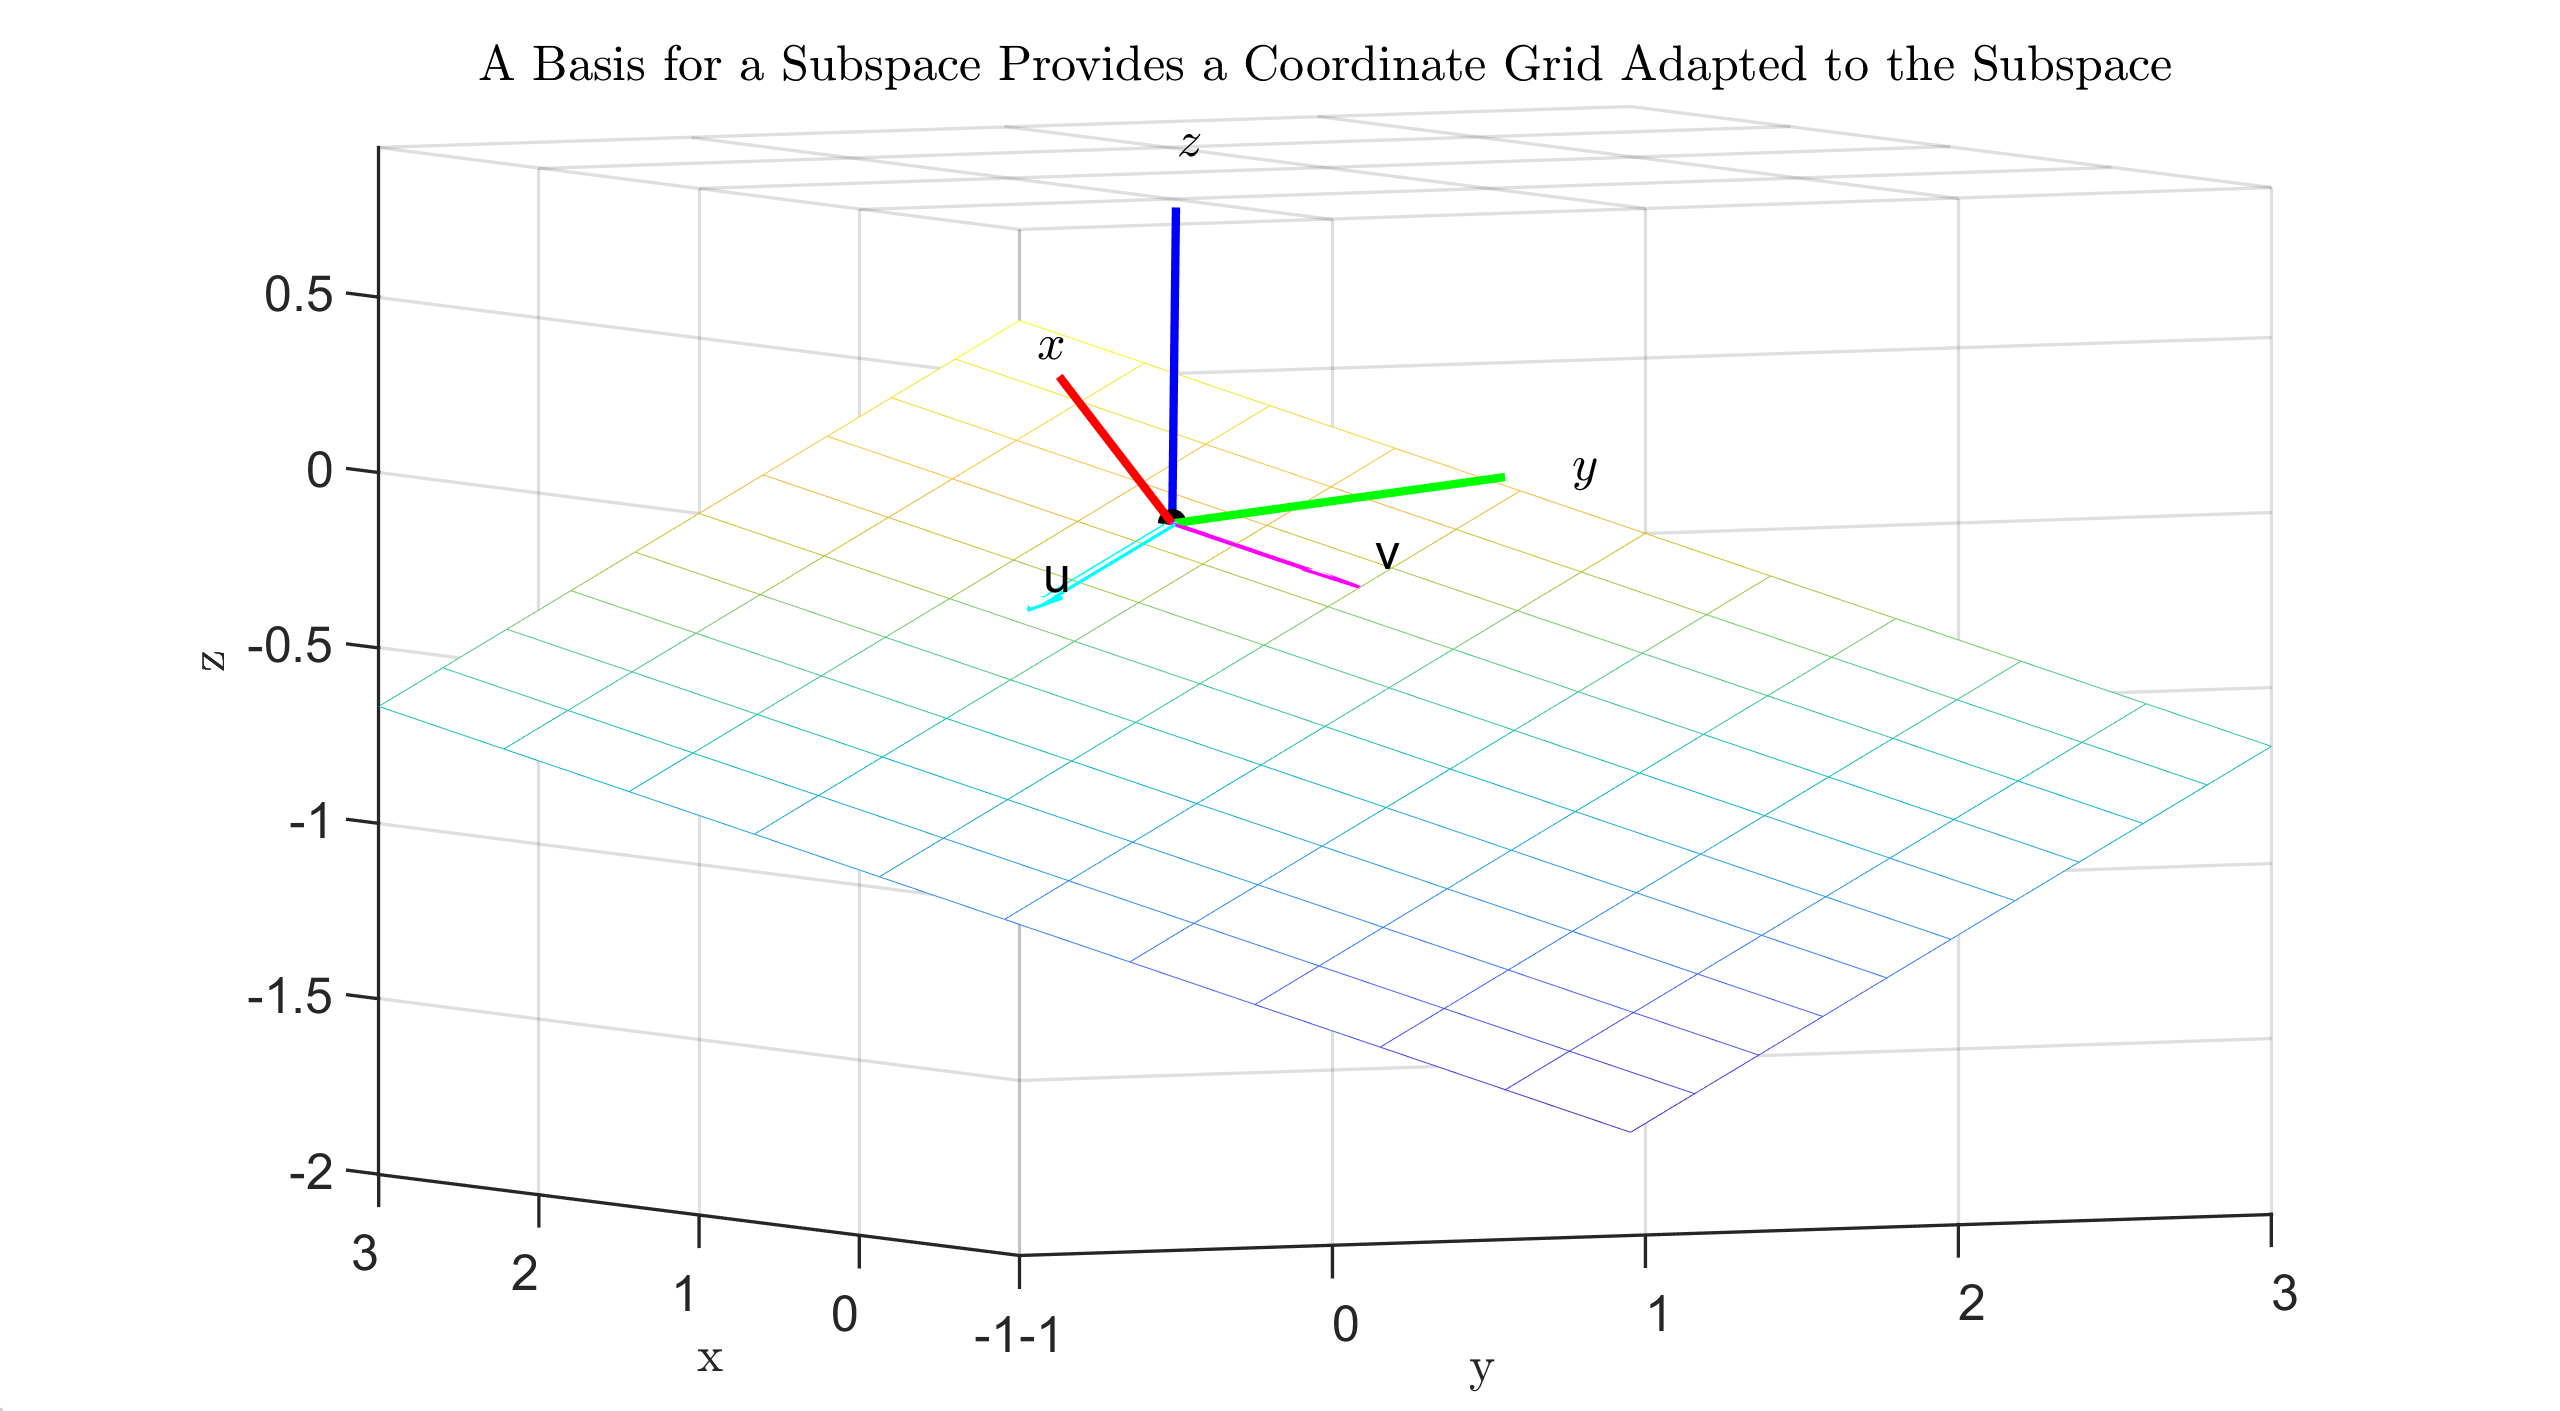
\includegraphics[width=0.75\textwidth]{graphics/Chap10Rn/SubspaceBasis.png}
\caption{This figure is an alternative representation of what we showed in Fig.~\ref{fig:Chap10Rn:CoordinatesNew}, namely $\real^3$ with a two-dimensional subspace (the gridded planar surface) $V$, this time with an orthogonal basis $\{u, v\}$. The natural basis $\{ e_1, e_2, e_3\}$, which gives the $(x, y, x)$ coordinates in $\real^3$, do not lie in $V$. \textbf{Hence, expressing locations in $V$ in terms of the ``natural coordinates'' from $\real^3$ is not very natural at all!} Because $V=\spanof{u, v}$, it is much simpler, and more natural, to express points in $V$ in terms of the basis vectors $u$ and $v$. Here, $u$ and $v$ were selected to be \textit{orthogonal}, but that is not a requirement. Any pair of linearly independent vectors in $V$ will work, as illustrated in Figures~\ref{fig:R2BasisVectors} and \ref{fig:R2BasisVectorsNotOrthognal}.}
    \label{fig:Chap10Rn:Coordinates}
\end{figure}



\begin{tcolorbox}[sharp corners, colback=green!30, colframe=green!80!blue, title=\textbf{\Large Vector Space Coordinates and Vector Representation}]
Suppose that $V$ is a $k$-dimensional subspace of $\real^n$ with basis $\{ v_1, v_2, \ldots, v_k\}$ or all of $\real^n$ itself (in which case, $k=n)$. Then each $x\in V$ can be expressed (uniquely) as a linear combination of basis vectors
\begin{equation}
    \label{eq:CoordinateExpansion}
    x = \alpha_1 v_1 + \alpha_2 v_2 + \cdots + \alpha_k v_k.
\end{equation}
Stacking the coefficients $\alpha_1 ,  \alpha_2,  \ldots,  \alpha_k$ into a column vector yields
\begin{equation}
    \label{eq:VectorRepresentation}
    [x]_{\{ v_1, \ldots, v_k\}} := \begin{bmatrix} \alpha_1 \\ \alpha_2 \\ \vdots \\ \alpha_k \end{bmatrix},
\end{equation}
which is called the \textbf{representation of $x$} in the basis $\{ v_1, v_2, \ldots, v_k\}$. The $k$-tuple 
 \begin{equation}
    \label{eq:Coordinates}
    \alpha: = \left(\alpha_1 ,  \alpha_2,  \ldots,  \alpha_k \right)
\end{equation}
forms the \textbf{coordinates of $x$} associated to the basis $\{ v_1, v_2, \ldots, v_k\}$. \\
\textbf{Remark:} We could just as easily written $ x = z_1 v_1 + z_2 v_2 + \cdots + z_k v_k,$ and then denoted our coordinates on $V$ as $z:=\left(z_1, z_2, \ldots, z_k  \right)$.
When you think of the coefficients in the linear combination as being constants, then denoting them as $\alpha_k$, $c_k$ or $a_k$ is rather common. If you are thinking of them as being variables, then denoting them as $x_k$, $y_k$, or $z_k$ is common. There is not fixed convention. 
\end{tcolorbox}



\begin{example}
\label{ex:FindBasisForGivenSubsapce} We consider the subspace of $\real^3$ defined by
$$V:=\left\{ x=\begin{bmatrix} x_1 \\x_2 \\x_3  \end{bmatrix} \in \real^3 ~|~ x_1+x_2+x_3=0 \right\}. $$
Show that $$ \left\{ v_1= \left[\begin{array}{r}
    1 \\ 0 \\ -1
\end{array}\right] , 
v_2= \left[\begin{array}{r}
    0 \\ 1 \\ -1
\end{array}\right]
\right\}  $$
is a basis for $V$ and hence $V$ is a two dimensional subspace of $\real^3$. In addition, show that 
$$ v:= \left[\begin{array}{r}
    3 \\ -4 \\ 1
\end{array}\right] \in V$$
and find its coordinates on $V$. 
\end{example}

\textbf{Solution:} To show that $\{v_1, v_2 \}$ is a basis for $V$, we need that to check that
\begin{itemize}
    \item $\{v_1, v_2 \} \subset V$,
    \item the set  $\{v_1, v_2 \}$ is linearly independent, and
    \item $\spanof{v_1, v_2 } =V$.
\end{itemize}
We leave the reader to show the first two properties: that $v_1$ and $v_2$ are in $V$ and they are linearly independent. The hard part is showing the span property, namely, that all vectors in $V$ can be written as a linear combination of $v_1$ and $v_2$. To do this, we note that
$$ x=\begin{bmatrix} x_1 \\x_2 \\x_3  \end{bmatrix} \in V \iff x_1+x_2+x_3=0 \iff x_3 = -(x_1 + x_2) \iff x= \begin{bmatrix} x_1 \\x_2 \\-(x_1 + x_2)  \end{bmatrix}.$$
Taking $x_1=1$ and $x_2 = 0$ gives $v_1$, while taking $x_1=0$ and $x_2 = 1$ gives $v_2.$ \\

We have 
$$ x=\begin{bmatrix} x_1 \\x_2 \\x_3  \end{bmatrix} \in V \iff  x= \begin{bmatrix} x_1 \\x_2 \\-(x_1 + x_2)  \end{bmatrix} \iff x = x_1 v_1 + x_2 v_2 \iff x \in \spanof{v_1, v_2}.$$

The dimension follows from the number of elements in the basis. \\

Now, we could just as easily have written
$$ x=\begin{bmatrix} x_1 \\x_2 \\x_3  \end{bmatrix} \in V \iff x_1+x_2+x_3=0 \iff x_2 = -(x_1 + x_3) \iff x= \begin{bmatrix} x_1 \\-(x_1 + x_3) \\x_3  \end{bmatrix}.$$
Then, taking $x_1=1$ and $x_3 = -1$ gives $v_1$, while taking $x_1=0$ and $x_3 = -1$ gives $v_2.$ \\

To complete the problem, we first verify that $v^\top = \left[\begin{array}{rrr}  3 & -4 & 1\end{array}\right]^\top $ is in $V$ because the sum of its components equals zero. Next, we check that
$$ v:= \left[\begin{array}{r}
    3 \\ -4 \\ 1
\end{array}\right] = 3 v_1 - 4 v_2$$
and hence its coordinates are $(3, -4)$ in the basis $\{v_1, v_2\}$.
\Qed\\

The point is that $V$ is now rather simple to understand and manipulate as the set of linear combinations of $v_1$ and $v_2$. Moreover, we can navigate within $V$ by using the natural coordinates induced by our choice of basis vectors. \\

The same idea applies to $\real^n$ itself. We are used to thinking of coordinates $\left(x_1, x_2, \ldots, x_n  \right)$ corresponding to the vector (or point) 
$$\left(x_1, x_2, \ldots, x_n  \right) \longleftrightarrow x_1 e_1 + x_2 e_2 + \cdots + x_n e_n = \left[\begin{array}{r}
    x_1 \\ x_2 \\ \vdots \\ x_n
\end{array}\right] ,$$ 
just as we did in \eqref{eq:R4ExampleBasis_b}. However, we are not obliged to use the natural basis vectors. We can in fact use any basis $\{ v_1, v_2, \ldots, v_n\}$ for $\real^n$ and express a vector $x$ in the new basis
$$\left(x_1, x_2, \ldots, x_n  \right) \longleftrightarrow x_1 e_1 + x_2 e_2 + \cdots + x_n e_n = z_1 v_1 + z_2 v_2 + \cdots + z_n v_n  \longleftrightarrow \left(z_1, z_2, \ldots, z_n  \right).$$ 


\vspace*{0.5cm}
\begin{tcolorbox}[sharp corners, colback=green!30, colframe=green!80!blue, title=\textbf{\Large Canonical or Natural Basis Vectors }] Let $n\ge1$ and, as before, define $e_i:= i$-th column of the $n \times n$ identity matrix, $I_n$. Then $$\{ e_1, e_2, \ldots, e_n\}$$ is a basis for the vector space $\real^n$. Its elements $e_i$ are called both \textbf{natural basis vectors} and \textbf{canonical basis vectors}. The frequency of usage of one name vs the other is about fifty-fifty!\\

\textbf{Remark:}  Showing linear independence is identical to \eqref{eq:R4ExampleBasis_a} and showing that the span is all of $\real^n$ is the same as in \eqref{eq:R4ExampleBasis_b}. 
\end{tcolorbox}
\vspace*{0.5cm}

\begin{tcolorbox}[title=\textbf{\Large Columns of Matrices and Bases of $\real^n$}]
We let $A$ be an $n\times n$ matrix. The following statements are equivalent
\begin{enumerate}
\renewcommand{\labelenumi}{(\alph{enumi})}
\setlength{\itemsep}{.2cm}
    \item $\det(A)\neq 0$.
    \item The columns of $A$ are linearly independent.
     \item The columns of $A$ form a basis for $\real^n$.
\end{enumerate}

\textbf{Remark:} As a special case, we can take $A = I_n$, the columns of which give the canonical basis vectors.
   
\end{tcolorbox}

\vspace*{.2cm}

\begin{example}
\label{ex:BasisR5} 
Determine if the vectors $\{v_1, \ldots, v_5\}$ form a basis for $\real^5$.
\begin{equation}
    \label{eq:NonorthognalBasis3R5}
    v_1=  \left[
\begin{array}{r}
1.0 \\
2.0 \\
0.0 \\
0.0 \\
2.0 \\
\end{array}
\right], v_2=\left[
\begin{array}{r}
-1.0 \\
0.0 \\
0.0 \\
1.0 \\
1.0 \\
\end{array}
\right], v_3= \left[
\begin{array}{r}
1.0 \\
2.0 \\
-2.0 \\
0.0 \\
2.0 \\
\end{array}
\right], v_4=\left[
\begin{array}{r}
0.0 \\
2.0 \\
-2.0 \\
0.0 \\
0.0 \\
\end{array}
\right], v_5=\left[
\begin{array}{r}
-1.0 \\
2.0 \\
0.0 \\
0.0 \\
2.0 \\
\end{array}
\right].
\end{equation}
 \end{example}

\textbf{Solution:}
We define
\begin{equation}
\label{eq:5by5matrix}
  A= \left[
\begin{array}{rrrrr}
1.0 & -1.0 & 1.0 & 0.0 & -1.0 \\
2.0 & 0.0 & 2.0 & 2.0 & 2.0 \\
0.0 & 0.0 & -2.0 & -2.0 & 0.0 \\
0.0 & 1.0 & 0.0 & 0.0 & 0.0 \\
2.0 & 1.0 & 2.0 & 0.0 & 2.0 \\
\end{array}
\right]_{5 \times 5} .
\end{equation}
In Julia, we compute $\det(A)=16.0$ and hence the set of vectors $\{v_1, \ldots, v_5\}$ does form a basis for $\real^5$.

\Qed

\begin{example}
\label{ex:BasisR5_partb} 
Compute a QR Factorization of $A$ in \eqref{eq:5by5matrix} and relate the vectors in \eqref{eq:NonorthognalBasis3R5}, that is, the columns of $A$, to the matrices $Q$ and $R$.
 \end{example}

\textbf{Solution:} We apply the Gram-Schmidt Process with Normalization to $\{v_1, \ldots, v_5\}$, the columns of $A$, and obtain
$$
Q=\left[
\begin{array}{rrrrr}
0.3333 & -0.6537 & 0.0000 & -0.4193 & -0.5345 \\
0.6667 & -0.1307 & 0.0000 & 0.7338 & 0.0000 \\
0.0000 & 0.0000 & -1.0000 & 0.0000 & 0.0000 \\
0.0000 & 0.5883 & 0.0000 & 0.1048 & -0.8018 \\
0.6667 & 0.4576 & 0.0000 & -0.5241 & 0.2673 \\
\end{array}
\right],~~R=\left[
\begin{array}{rrrrr}
3.0000 & 0.3333 & 3.0000 & 1.3333 & 2.3333 \\
0.0000 & 1.6997 & 0.0000 & -0.2615 & 1.3074 \\
0.0000 & 0.0000 & 2.0000 & 2.0000 & 0.0000 \\
0.0000 & 0.0000 & 0.0000 & 1.4676 & 0.8386 \\
0.0000 & -0.0000 & 0.0000 & 0.0000 & 1.0690 \\
\end{array}
\right].
$$
By construction, the columns of $Q$ form an orthonormal basis for $\spanof{v_1, \ldots, v_5}=:\colspanof{A}$. Indeed, we let  $\{q_1, \ldots, q_5\}$ denote the columns of $Q$ and then verify that
$$v_1 = 3 q_1, v_2 = 0.33 q_1 + 1.7 q_2, v_3 = 3 q_1 + 3 q_3, v_4 =  1.33 q_1 - 0.26 q_2 + 2.0 q_3 + 1.47 q_4, v_5 = 2.22 q_1 + 1.31 q_2 + 0.84 q_4 + 1.07 q_5,$$
confirming what we know from Gram-Schmidt, namely that
$$\spanof{v_1, \ldots, v_5} = \spanof{q_1, \ldots, q_5}. $$

\Qed

\vspace*{.2cm}

\textbf{(Optional Read):} Proof the Facts $(a) \iff (b) \iff (c)$  for Columns of Matrices and Bases of $\real^n$.\\

$(a) \iff (b)$. 
%We assume that $\det(A)\neq0$ and must show that the columns of $A$ are linearly independent. 
We denote the columns of $A$ by $\{v_1=a^{\rm col}_1, v_2=a^{\rm col}_2, \ldots, v_n=a^{\rm col}_n \}$. The columns of $A$ are linearly independent if, and only if, the unique solution to
\begin{equation}
    \label{eq:LinearIdepForBasisProof}
    \alpha_1 a^{\rm col}_1 +  \alpha_2 a^{\rm col}_2 + \cdots + \alpha_n a^{\rm col}_n = 0_{n \times 1}
\end{equation}
is the trivial solution, $\alpha_1=0, \alpha_2=0, \ldots, \alpha_n=0$.
But this is equivalent to
\begin{align*}
   \underbrace{ \left[ a^{\rm col}_1 ~~a^{\rm col}_2~~a^{\rm col}_n \right]}_{A} \underbrace{\left[\begin{array}{c} \alpha_1 \\ \alpha_2 \\ \vdots \\ \alpha_n  \end{array}  \right]}_{\alpha} &= 0_{n \times 1}\\
   & \Updownarrow \\
   A \alpha &= 0_{n \times 1}
\end{align*}
When $A$ is square, we know that $\det(A) \neq 0$ if, and only if, the unique solution to $A\alpha = 0$ is the trivial solution $\alpha = 0_{n \times 1}$\\

 $(b) \iff (c)$. The direction $(c) \implies (b)$ is trivial, hence we only need to show that  $(b) \implies (c)$ To do so, we assume that $A$ is $n \times n$ and its columns are linearly independent, and must show that they span $\real^n$, that is, we must show that
$$\spanof{ v_1, v_2,  \ldots, v_n}= \real^n. $$
Well, spans are simply linear combinations, so the question becomes, can every vector in $b \in \real^n$ be written as a linear combination of the columns of $A$? Because the dimension of $\real^n$ equals $n$, we know that the set 
$$\{b,  v_1, v_2,  \ldots, v_n  \} $$
is linearly dependent. Hence, there there exist coefficients $\alpha_0,  \ldots, \alpha_n$ not all zero such that 
$$ \alpha_0 b + \alpha_1 v_1 + \alpha_2 v_2 + \cdots \alpha_n v_n =0.$$
We observe that if $\alpha_0 \neq 0$, because if it were zero, then
$$ \alpha_1 v_1 + \alpha_2 v_2 + \cdots \alpha_n v_n =0,$$
which is not possible because $\{ v_1, v_2,  \ldots, v_n\}$ is linearly independent. Hence, we have that
$$ b=-\frac{\alpha_1}{\alpha_0} v_1 -\frac{\alpha_2}{\alpha_0} v_2 - \cdots -\frac{\alpha_n}{\alpha_0} v_n,$$
proving that $b \in \spanof{ v_1, v_2,  \ldots, v_n}$.
\Qed 


% \vspace*{.4cm}

% \textit{The following brings together--into one place--everything we know for \textbf{square} systems of equations.}\\

% \begin{tcolorbox}[sharp corners, colback=green!30, colframe=green!80!blue, title=\textbf{\Large A Potpourri of Facts about Square Systems of Linear Equations}] Let $A$ be an $n\times n$ matrix and associate its column with vectors in $\real^n$ by $\{v_1=a^{\rm col}_1, v_2=a^{\rm col}_2, \ldots, v_n=a^{\rm col}_n \}$. Then the following statements are equivalent:
% \begin{itemize}
%     \item for every vector $b \in \real^n$, the equation $Ax=b$ has a unique solution;
%         \item $\det(A) \neq 0$;
%     \item the set $\{v_1, v_2, \ldots, v_n \}$ is linearly independent;
%     \item the set $\{v_1, v_2, \ldots, v_n \}$ is a basis of $\real^n$;
%     \item $\colspanof{A} = \real^n$;
%     \item for every vector $b \in \real^n$, the equation $Ax=b$ has a solution;
%     \item for some vector $b \in \real^n$, the equation $Ax=b$ has a solution and it is unique; and
%         \item the equation $Ax=0_{n \times 1}$ has a unique solution.
% \end{itemize}
% \end{tcolorbox}

% Can you piece together all of these facts? If not, let the leader of your recitation section know, or, work with student colleagues on Piazza!


\section{Eigenvalues and Eigenvectors}

For a first introduction to eigenvalues and eigenvectors, this video by 3Blue1Brown is quite good\footnote{In the video, when they talk about $\hat{i}$, they mean our natural basis vector $e_1$, and when they say $\hat{j}$, they mean our natural basis vector $e_2$ }: \url{https://www.youtube.com/watch?v=PFDu9oVAE-g}. Here, we provide a cursory introduction to the topic, hitting only some of the highlights. A more thorough treatment is given in Appendices~\ref{sec:CaseEigenvectors} and~\ref{sec:EigenStuff}. \\

What does ``eigen'' even mean? From Quora, ``eigen'' is a German word that in English means ``own'', ``unique to'', ``peculiar to'', or ``characteristic of'' the originating matrix. Your author likens it to the English word \textit{self}. A non-zero vector $v \in \real^n$ such that when you multiply it by an $n \times n$ matrix you basically get the vector \textit{itself} back, is called an \textit{eigenvector}, or a self-vector. Exactly the same vector back? No, but almost! An \textit{eigenvector} $v$ satisfies $A v = \lambda v$, with $\lambda$ being a scalar called the \textit{eigenvalue}, or self-value. The exactly true ``itself'' part is that whenever $\lambda \neq 0$
$$\spanof{A v} = \spanof{v}.$$
It's kind of amazing to contemplate: an $n \times n$ matrix has $n^2$ entries so how is it even possible that there are non-zero $n \times 1$-vectors such that $A v = \lambda v$, without $A$ being something trivial like a constant times an identity matrix? \\

% \textbf{Motivation:} For an $n\times n$ matrix $A$ with real coefficients, we can define a function 
% $$ f: \real^n \to \real^n$$
% by $f(x):=Ax$. That is, for $x \in \real^n$, the function $f(x)$ returns the value $Ax$, which is another vector in $\real^n$ because we assumed $A$ to be $n \times n$. 

In fact, when we multiply a matrix times a vector, we expect the terms to get all jumbled up. For example, we know that
$$\left[\begin{array}{rrc}  a_{11} & a_{12} & a_{13} \\  a_{21} & a_{22} & a_{23}  \\ a_{31} & a_{32} & a_{33} \end{array} \right] \left[\begin{array}{r}  x_1 \\ x_2 \\ x_3\end{array} \right] = \left[\begin{array}{r}  a_{11} x_1 + a_{12} x_2 + a_{13} x_3 \\  a_{21} x_1 + a_{22} x_2 + a_{23} x_3 \\  a_{31} x_1 + a_{32} x_2 + a_{33} x_3\end{array} \right],$$
and thus it is very hard to imagine that we could have 
$$\left[\begin{array}{rrc}  a_{11} & a_{12} & a_{13} \\  a_{21} & a_{22} & a_{23}  \\ a_{31} & a_{32} & a_{33} \end{array} \right] \left[\begin{array}{r}  x_1 \\ x_2 \\ x_3\end{array} \right] = \lambda \left[\begin{array}{r}  x_1 \\ x_2 \\ x_3\end{array} \right]$$
for some ``magical values'' of $x_1, x_2$ and $x_3$. 



\vspace*{.2cm}

\begin{figure}[h]%
\centering
\subfloat[]{%
    \label{fig:MotivateEigenvectorsA}%
	\centering
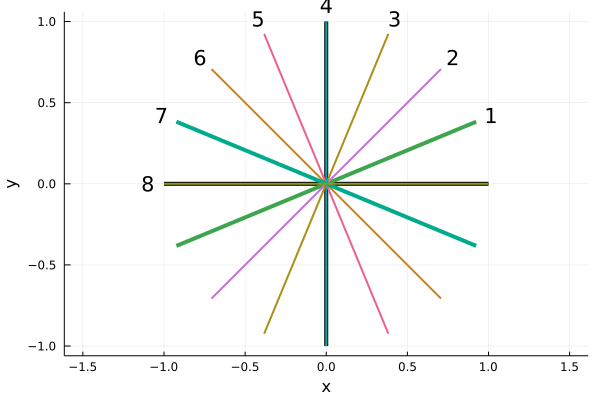
\includegraphics[width=0.45\columnwidth]{graphics/Chap10Rn/MotivateEigenvectors.png}}%
\hspace{5pt}%
\subfloat[]{%
    \label{fig:MotivateEigenvectorsB}%
	\centering
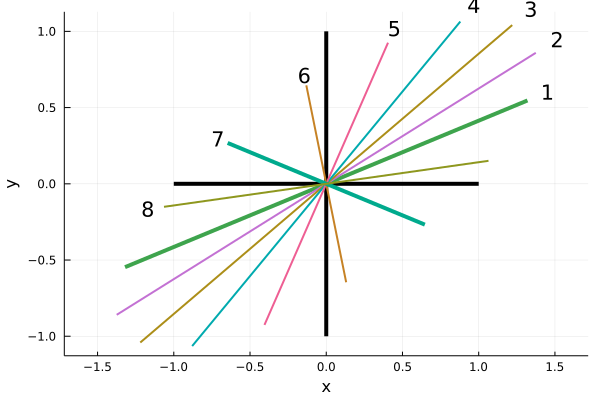
\includegraphics[width=0.45\columnwidth]{graphics/Chap10Rn/MotivateEigenvectorsB.png}}%
    \caption[]{Matrices tend to both rotate and scale vectors, and at firt blush, the amount of rotation and scaling is seemingly hard to predict. (a) Shows a set of eight vectors $v_i \in \real^2$, with each vector having length one. We've also plotted the negative of each vector so that you can more easily visualize their span as one-dimensional subspaces in $\real^2$. (b) Shows the vectors $A v_i$ for a $2 \times 2$ matrix $A$ given in Example~\ref{ex:EigenVectorsR2}. If you look carefully, you will see that vectors $\{v_1, v_7 \}$ are not rotated by $A$; they are only scaled. Indeed $Av_1 = 1.4 v_1$ and $Av_7 = 0.7 v_7$. The remaining vectors $\{ v_2, v_3, v_4, v_5, v_6, v_8 \}$ are both rotated and scaled. Non-zero vectors that satisfy $Av = \lambda v$ are called \textit{eigenvectors} of $A$ and $\lambda$ is called an \textit{eigenvalue}. Comparing Figures (a) and (b), we observe that $\spanof{A v_1} =\spanof{v_2}$ and $\spanof{A v_7} =\spanof{v_7}$.
    }
    \label{fig:MotivateEigenvectorsEigenvalues}
\end{figure}


\begin{example} \label{ex:EigenVectorsR2}
For the matrix 
$
A:=\left[
\begin{array}{cc}
1.0643 & 0.8795 \\
0.1509 & 1.0643 \\
\end{array}
\right]
$
and the vectors $\{v_1, v_2, \ldots, v_8 \}$ plotted in Fig.~\ref{fig:MotivateEigenvectorsEigenvalues}, compute $A v_i$ and check if you can find a real constant $\lambda_i$ such that $Av_i = \lambda_i v_i$.
%%%$\{A v_1, Av_2, \ldots, Av_8 \}$.
\end{example}
\vspace*{.3cm}

\textbf{Solution:} We first give the vectors and immediately below them, their multiplication by $A$.

\begin{equation}
\underbrace{
\left[
\begin{array}{r}
0.9239 \\
0.3827 \\
\end{array}
\right]}_{v_1}, \underbrace{
\left[
\begin{array}{r}
0.7071 \\
0.7071 \\
\end{array}
\right]}_{v_2}, \underbrace{
\left[
\begin{array}{r}
0.3827 \\
0.9239 \\
\end{array}
\right]}_{v_3}, \underbrace{
\left[
\begin{array}{r}
0.0000 \\
1.0000 \\
\end{array}
\right]}_{v_4},  \underbrace{
\left[
\begin{array}{r}
-0.3827 \\
0.9239 \\
\end{array}
\right]}_{v_5},  \underbrace{
\left[
\begin{array}{r}
-0.7071 \\
0.7071 \\
\end{array}
\right]}_{v_6},  \underbrace{
\left[
\begin{array}{r}
-0.9239 \\
0.3827 \\
\end{array}
\right]}_{v_7}, \underbrace{
\left[
\begin{array}{r}
-1.0000 \\
0.0000 \\
\end{array}
\right]}_{v_8}
\end{equation}

\vspace*{.2cm}
\begin{equation}
\underbrace{
\left[
\begin{array}{r}
1.3198 \\
0.5467 \\
\end{array}
\right]}_{A v_1}, \underbrace{
\left[
\begin{array}{r}
1.3744 \\
0.8593 \\
\end{array}
\right]}_{A v_2}, \underbrace{
\left[
\begin{array}{r}
1.2198 \\
1.0410 \\
\end{array}
\right]}_{A v_3}, \underbrace{
\left[
\begin{array}{r}
0.8795 \\
1.0643 \\
\end{array}
\right]}_{A v_4}, \underbrace{
\left[
\begin{array}{r}
0.4052 \\
0.9255 \\
\end{array}
\right]}_{A v_5},   \underbrace{
\left[
\begin{array}{r}
-0.1307 \\
0.6459 \\
\end{array}
\right]}_{A v_6}, \underbrace{
\left[
\begin{array}{r}
-0.6467 \\
0.2679 \\
\end{array}
\right]}_{A v_7}, \underbrace{
\left[
\begin{array}{r}
-1.0643 \\
-0.1509 \\
\end{array}
\right]}_{A v_8}
\end{equation}

\vspace*{.2cm}
For there to exist $\lambda_1$ such that $Av_1 = \lambda_1 v_1$, we know from the first rows of $v_1$ and $Av_1$ that their ratio is $1.3198/0.9239 \approx 1.4$; we further check that the same ratio holds for the second components, and hence $Av_1 = 1.4 v_1$. We'll leave it to the reader to apply the same method on the remaining vectors and verify that $Av_7 = 0.7 v_7$, while none of the other vectors satisfies $A v_i = \lambda_i v_i$ for some scalar $\lambda_i$.
\Qed

\vspace*{.2cm}
\begin{example} Multiply the matrix 
\begin{equation}
A:=\left[
\begin{array}{rrr}
-8.0 & 10.0 & 10.0 \\
-2.0 & 5.0 & 2.0 \\
-10.0 & 9.0 & 12.0 \\
\end{array}
\right]
\end{equation}
times each of the vectors $\{v_1, v_2, v_3 \}$, where 
\begin{equation}
v_1=\left[
\begin{array}{r}
1.0 \\
0.0 \\
1.0 \\
\end{array}
\right],~v_2=\left[
\begin{array}{r}
0.0 \\
-1.0 \\
1.0 \\
\end{array}
\right], \text{ and } v_3=\left[
\begin{array}{c}
5.0 \\
2.0 \\
4.0 \\
\end{array}
\right].
\end{equation}

\end{example}

\textbf{Solution:} It's more impressive if you do the required multiplications by hand, but turning to Julia we obtain
\begin{equation}
A v_1 = \left[
\begin{array}{r}
2.0 \\
0.0 \\
2.0 \\
\end{array}
\right] = \mathbf{2} v_1, ~A v_2 = \left[
\begin{array}{r}
0.0 \\
-3.0 \\
3.0 \\
\end{array}
\right] = \mathbf{3} v_2, \text{ and } A v_3 = \left[
\begin{array}{r}
20.0 \\
8.0 \\
16.0 \\
\end{array}
\right] = \mathbf{4} v_3.
\end{equation}
Hence, when $A$ acts on this set of vectors, all it does is scale the vector by a factor of 2, 3 or 4, respectively. There is no ``rotation'' of the vector. That seems kind of magical. 
%In addition, we check 
% A (-5 v_3)=\begin{equation}
% \left[
% \begin{array}{r}
% -100.0 \\
% -40.0 \\
% -80.0 \\
% \end{array}
% \right] = 4(-5 v_3)
% \end{equation}, 
% verifying that if $A v = \lambda v$, then $A (\alpha v) = \lambda (\alpha v). $
\Qed



\vspace*{.2cm}

\begin{tcolorbox}[title=\textbf{\Large Eigen Stuff: Temporary Definitions}]
 Let $A$ be an $n\times n$ matrix with real coefficients. A scalar $\lambda \in \real$ is an \textbf{eigenvalue} of $A$, if there exists a non-zero vector $v \in \real^{n}$ such that $A  v=\lambda v$. Any such vector $v$ is called an \textbf{eigenvector} associated with $\lambda$. We note that if $v$ is an eigenvector, then so is $\alpha v$ for any $\alpha \neq 0$, and therefore, eigenvectors are not unique. The true definition is given in Appendix~\ref{sec:EigenStuff}.
\end{tcolorbox}

\vspace*{.2cm}

To find eigenvalues, we need to have conditions under which there exists $v \in \real^n$, $v \neq 0$, such that $A v=\lambda v$. We first note that 
$$A  v=\lambda v \iff \lambda v -Av = 0_{n \times 1} \iff \lambda I v -Av = 0_{n \times 1}  \iff(\lambda I-A) v=0_{n \times 1}.$$
We then note that there exists $v \neq 0_{n \times 1}$ such that $(\lambda I-A) v=0_{n \times 1}$ if, and only if 
    \begin{equation*}
   \det(\lambda I-A)=0.
    \end{equation*}
    
    \begin{example}
\label{ex:Chap10Eigen01} Let $A$ be the $2 \times 2$ real matrix
 $A=\left[\begin{array}{rr}
    1 & 2\\
    3 & 2
    \end{array}\right].$
Determine, if any, its eigenvalues and eigenvectors. 
\end{example}

\textbf{Solution:} To find eigenvalues, we need to solve 
$$\det(\lambda I-A)= \left| \begin{array}{cc}
    \lambda-1 & -2\\
   -3 &\lambda -2
    \end{array} \right| =(\lambda-1)(\lambda-2)-6=\lambda^2- 3 \lambda -4=0.$$
    We compute the discriminant of this quadratic equation and we find
    $$b^2-4ac = 9 +16 =25 >0,$$
    and therefore there are two real solutions. We compute them with the quadratic formula to be $\lambda_1=-1$ and $\lambda_2=4$.\\
    
   To determine an eigenvector associated with $ \lambda_1=-1$, we need to find $v_1\in \real^2$ such that 
   \begin{align*}
       (A-\lambda_1 I_2) v_1 & = 0_{2 \times 1}\\
        & \Updownarrow \\
   \left( \left[\begin{array}{rr}
    1 & 2\\
    3 & 2
    \end{array}\right] - (-1)   \left[\begin{array}{rr}
    1 & 0\\
    0& 1
    \end{array}\right]\right) \left[\begin{array}{r}
   v_{1a} \\
  v_{1b}
    \end{array}\right] & = \left[\begin{array}{r}
   0 \\
  0
    \end{array}\right]\\
     & \Updownarrow \\
      \left[\begin{array}{rr}
    2 & 2\\
    3 & 3
    \end{array}\right]  \left[\begin{array}{r}
   v_{1a} \\
  v_{1b}
    \end{array}\right] & = \left[\begin{array}{r}
   0 \\
  0
    \end{array}\right]\\
    & \Updownarrow \\
   \left[\begin{array}{r}
   v_{1a} \\
  v_{1b}
    \end{array}\right] & = \alpha_1  \left[\begin{array}{r}
   1 \\
  -1
    \end{array}\right], ~\alpha_1 \neq 0.
   \end{align*}
  
   Similarly, to determine an eigenvector associated with $ \lambda_2=4$, we need to find $v_2\in \real^2$ such that 
   \begin{align*}
       (A-\lambda_2 I_2) v_2 & = 0_{2 \times 1}\\
        & \Updownarrow \\
   \left( \left[\begin{array}{rr}
    1 & 2\\
    3 & 2
    \end{array}\right] - (4)   \left[\begin{array}{rr}
    1 & 0\\
    0& 1
    \end{array}\right]\right) \left[\begin{array}{r}
   v_{2a} \\
  v_{2b}
    \end{array}\right] & = \left[\begin{array}{r}
   0 \\
  0
    \end{array}\right]\\
     & \Updownarrow \\
      \left[\begin{array}{rr}
    -3 & 2\\
    3 & -2
    \end{array}\right]  \left[\begin{array}{r}
   v_{2a} \\
  v_{2b}
    \end{array}\right] & = \left[\begin{array}{r}
   0 \\
  0
    \end{array}\right]\\
    & \Updownarrow \\
   \left[\begin{array}{r}
   v_{2a} \\
  v_{2b}
    \end{array}\right] & = \alpha_2  \left[\begin{array}{r}
   2\\
 3
    \end{array}\right], ~\alpha_2 \neq 0.
   \end{align*}
    

\Qed

\vspace*{.3cm}

\begin{tcolorbox}[title=\textbf{\Large Finding Eigenvectors and Eigenvalues with Julia}]
Beyond $2 \times 2$ matrices, we do not compute eigenvalues or eigenvectors by hand! In ROB 101, we use Julia!

\begin{lstlisting}[language=Julia,style=mystyle]
Random.seed!(876543212345678);
B=randn(4,4)
A=B'*B # symmetric matrices have real eigenvalues

E=eigen(A)
@show E.values
E.vectors
\end{lstlisting} 
\end{tcolorbox}
\textbf{Output} 
\begin{verbatim}
E.values = [0.06287200462929299, 0.6813033999332612, 2.9738855645273268, 4.4839915456638]

4 x 4  Matrix{Float64}:
  0.339074   0.0385456  -0.71411   -0.61122
  0.551488   0.528452   -0.226828   0.604275
 -0.191731   0.824533    0.318536  -0.426521
  0.737651  -0.19849     0.58063   -0.281676
\end{verbatim}


\vspace*{.3cm}
    
    
\begin{example}
\label{ex:Chapt10EigenComplex} Let $A$ be the $2 \times 2$ real matrix
 $A=\left[\begin{array}{rr}
    0 & 1\\
    -1 & 0
    \end{array}\right].$
Using our temporary definition, determine, if any, its eigenvalues and eigenvectors. 
\end{example}

\textbf{Solution:} To find eigenvalues, we need to solve 
$$\det(\lambda I-A)= \left| \begin{array}{rr}
    \lambda & -1\\
    1 &\lambda
    \end{array} \right| =\lambda^2+1=0.$$
    We compute the discriminant of this quadratic equation and we find
    $$b^2-4ac = -4 <0,$$
    and therefore there are no real solutions. Hence, by our \textit{temporary definition}, this $2 \times 2$ real matrix does not have any eigenvalues, and hence, neither does it have any eigenvectors.\\
\Qed
\vspace*{.5cm}

\begin{tcolorbox}[title=\textbf{\Large Full Story on Eigenstuff}]
\textbf{The correct definition of eigenvalues and eigenvectors requires complex numbers.} Example~\ref{ex:Chapt10EigenComplex} shows that if we allow eigenvalues to be complex numbers, then we'll have two eigenvalues corresponding to the two complex solutions of the quadratic equation $\lambda^2+1=0$, namely, $\lambda_1 = \im$ and $\lambda_2 = -\im$. As illustrated in Example~\ref{ex:Chap10Eigen02}, when seeking solutions to $(A-\lambda_i) v_i = 0$, you'll find that you need to allow the eigenvectors to have complex entries as well. \\ 

The full and correct treatment of eigenstuff is given in Appendices~\ref{sec:CaseEigenvectors} and~\ref{sec:EigenStuff}. Here, we are giving you a simplified treatment.
 \end{tcolorbox}   


\begin{example}
\label{ex:Chap10Eigen02} (Optional Read:) Let $A$ be the $2 \times 2$ real matrix that we treated in Example~\ref{ex:Chapt10EigenComplex}, namely,
 $A=\left[\begin{array}{rr}
    0 & 1\\
    -1 & 0
    \end{array}\right].$
Determine its eigenvalues and eigenvectors in the sense of Appendix~\ref{sec:EigenStuff}. 
\end{example}

\textbf{Solution:} As in Example~\ref{ex:Chapt10EigenComplex}, to find eigenvalues, we solve 
$$\det(\lambda I-A)= \left| \begin{array}{rr}
    \lambda & -1\\
    1 &\lambda
    \end{array} \right| =\lambda^2+1=0.$$
   We apply the quadratic equation and determine $\lambda_1 = \im$ and $\lambda_2= - \im$.  To find the eigenvectors, we solve 
   $$(A-\lambda_{i}I)v_i=0.$$
    The eigenvectors are $$v_{1}=\left[\begin{array}{c}
        1\\
        \im
    \end{array}\right],v_{2}=\left[\begin{array}{c}
        1\\
        -\im
    \end{array}\right].$$
Note that the eigenvalues and eigenvectors each form complex conjugate pairs. Indeed,
$$\lambda_2 = \lambda_1^\ast~~\text{and}~~v_2 = v_1^\ast. $$
\Qed

\vspace*{0.5cm}
\begin{tcolorbox}[sharp corners, colback=green!30, colframe=green!80!blue, title=\textbf{\Large When the Eigenvalues are Real and Distinct, the Eigenvectors form a Basis of $\real^n$}]
Let $A$ be an $n \times n$ matrix with real coefficients. If the eigenvalues $\{ \lambda_1,\ldots, \lambda_n \}$ are real and \textbf{distinct}, that is, $\lambda_i \neq \lambda_j $ for all $1 \le i \neq j \le n$, then the eigenvectors $\{ v_1,\ldots,v_n \}$ are real and provide a basis of $\real^n.$\\

Once again, the full story is given in Appendices~\ref{sec:CaseEigenvectors} and~\ref{sec:EigenStuff}. An interesting tidbit is that symmetric matrices always have real eigenvalues. Moreover, their eigenvectors can always be selected to form an orthogonal matrix; see Appendix~\ref{sec:RealSymmetricMatrices}.
\end{tcolorbox}

\vspace*{0.5cm}

\begin{example}
\label{ex:BasisEigenvectors}
Using Julia, find the eigenvalues and eigenvectors of the $3 \times 3$ (symmetric) matrix below. Furthermore, determine if the eigenvectors form a basis of $\real^3$.

\begin{equation}
A:=\left[
\begin{array}{rrr}
2.2216 & 1.6798 & -0.2670 \\
1.6798 & 0.8457 & -0.1651 \\
-0.2670 & -0.1651 & 0.6391 \\
\end{array}
\right].
\end{equation}
\end{example}

\textbf{Solution:} 
\begin{lstlisting}[language=Julia,style=mystyle]
E=eigen(A)
E.values
E.vectors
det(E.vectors)
\end{lstlisting}
Using Julia, we compute that 
\begin{equation}
\left[
\begin{array}{rrr}
\lambda_1&
\lambda_3 &
\lambda_3
\end{array}
\right] =\left[
\begin{array}{rrr}
-0.2817 &
0.6034 &
3.3848 
\end{array}
\right] \text{ and } \left[
\begin{array}{rrr}
v_1&
v_3 &
v_3
\end{array}
\right] =
\left[
\begin{array}{rrr}
0.5581 & 0.0870 & -0.8252 \\
-0.8297 & 0.0741 & -0.5533 \\
0.0131 & 0.9934 & 0.1135 \\
\end{array}
\right].
\end{equation}
Because the eigenvalues are distinct, we know that set $\{v_1, v_2, v_3 \}$ forms a basis of $\real^3$. To double check this, we determine that $\det(E.vectors)=1 \neq 0$ so that indeed, the eigenvectors are linearly independent and hence form a basis. 
\Qed

\vspace*{0.2cm}

\begin{figure}[h]%
\centering
\subfloat[]{%
    \label{fig:SquishingSpacea}%
	\centering
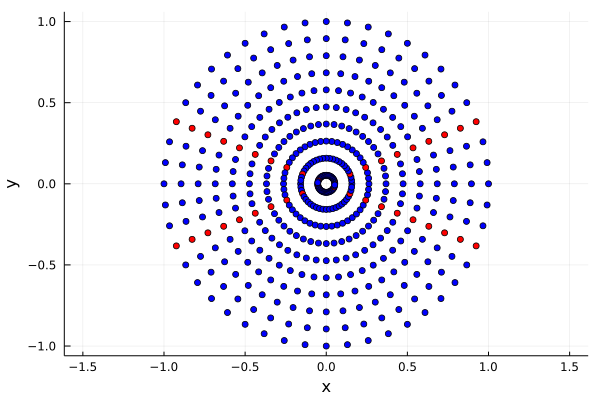
\includegraphics[width=0.45\columnwidth]{graphics/Chap10Rn/SquishingSpaceA.png}}%
\hspace{5pt}%
\subfloat[]{%
    \label{fig:SquishingSpaceb}%
	\centering
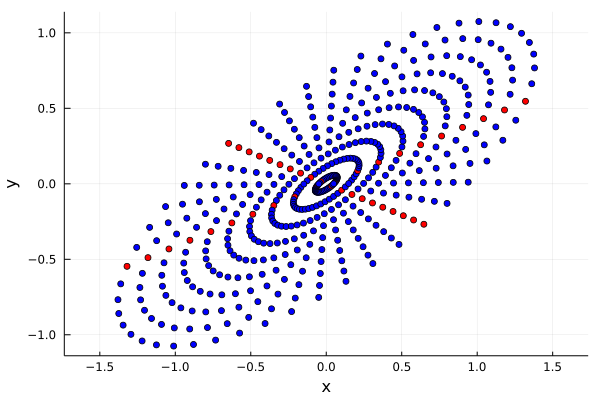
\includegraphics[width=0.45\columnwidth]{graphics/Chap10Rn/SquishingSpaceB.png}}%
\hspace{5pt}%
    \subfloat[]{%
    \label{fig:SquishingSpacec}%
	\centering
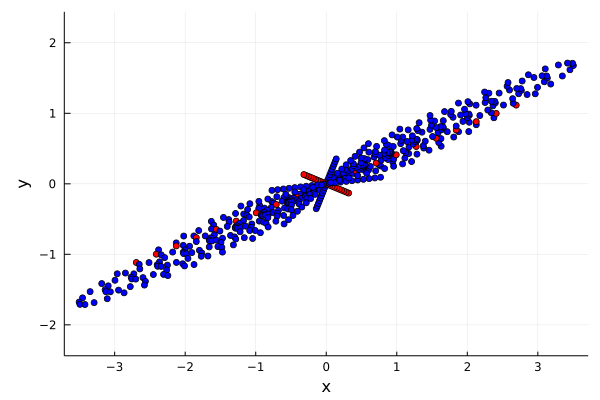
\includegraphics[width=0.45\columnwidth]{graphics/Chap10Rn/SquishingSpaceC.png}}%
\hspace{5pt}%
\subfloat[]{%
    \label{fig:SquishingSpaced}%
	\centering
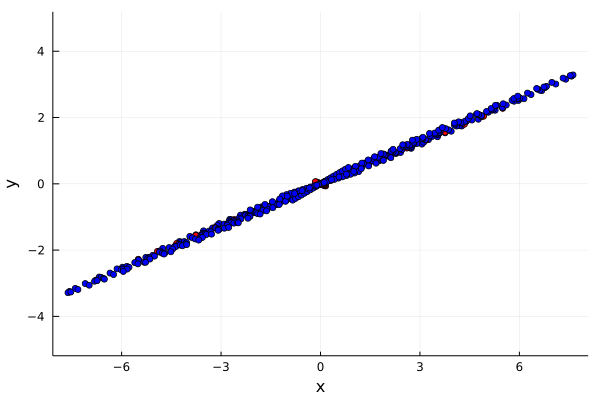
\includegraphics[width=0.45\columnwidth]{graphics/Chap10Rn/SquishingSpaceD.png}}%
    \caption[]{The data for this figure come from Example~\ref{ex:EigenVectorsR2}. The matrix $A$ is  $2 \times 2$ and has real eigenvalues and eigenvectors that satisfy $Av_1 = 1.4 v_1$ and $A v_2 = 0.7 v_2$. $A$ is ``expanding'' in the direction $v_1$ and ``contracting'' in the direction $v_2$. (a) Shows a uniform distribution of points, with the two eigenvectors highlighted in red. (b) For each point $x$ in the grid of (a), (b) shows it's image $Ax$. The circle is being squished into an ellipse under the action of $A$. This phenomenon is accentuated in (c), which shows $A^3 x$, and even more so in (d), which shows $A^5 x$. If we looked at $A^n x$ as $n \to \infty$, all of the points would lie on the ``expanding'' eigenvector, $v_1$.
    }
    \label{fig:SquishingSpace}
\end{figure}

\vspace*{.2cm}
\begin{tcolorbox}[sharp corners, colback=green!30, colframe=green!80!blue, title=\textcolor{red}{\Large \bf Utility of Eigenvalues and Eigenvectors:} \textbf{\Large They Explain how a Square Matrix acts on a Vector}]
Let $A$ be an $n \times n$ real matrix with real eigenvalues $\{ \lambda_1,\ldots, \lambda_n \}$ that are \textbf{distinct}, that is, $\lambda_i \neq \lambda_j $ for all $1 \le i \neq j \le n$. It then follows that the eigenvectors $\{ v_1,\ldots,v_n \}$ provide a basis for $\real^n.$ Let $x\in \real^n$ be arbitrary and write it as a linear combination of the basis of eigenvectors
\begin{equation}
    \label{eq:xExpandedEigenBasis}
    x = \alpha_ 1 v_1 + \alpha_2 v_2 + \cdots + \alpha_n v_n.
\end{equation}
Then because $Av_i = \lambda_i v_i$,
\begin{equation}
    \label{eq:xExpandedEigenBasisA}
   A x = \alpha_ 1 \lambda_1 v_1 + \alpha_2 \lambda_2 v_2 + \cdots +\alpha_n  \lambda_n v_n.
\end{equation}
If we apply $A$ to both sides of \eqref{eq:xExpandedEigenBasisA}, we obtain
\begin{equation}
    \label{eq:xExpandedEigenBasisA2}
    \begin{aligned}
       A^2 x &= \alpha_ 1 \lambda_1 A v_1 + \alpha_2 \lambda_2 A v_2 + \cdots +\alpha_n  \lambda_n Av_n \\
       &= \alpha_ 1 (\lambda_1)^2 v_1 + \alpha_2 (\lambda_2)^2  v_2 + \cdots +\alpha_n  (\lambda_n)^2 v_n,
    \end{aligned}
\end{equation}
where $A^2:= A \cdot A$ and we have used again, $A v_i = \lambda_i v$. 
Moreover, using this fact iteratively yields that, for all $k \ge 2$,
\begin{equation}
    \label{eq:xExpandedEigenBasisB}
   A^k x = \alpha_ 1 (\lambda_1)^k v_1 + \alpha_2 (\lambda_2)^k v_2 + \cdots +\alpha_n  (\lambda_n)^k v_n.
\end{equation}

\end{tcolorbox}
\vspace*{.3cm}

\textbf{Remarks:} 
\begin{itemize}
    \item Equation \eqref{eq:xExpandedEigenBasisB} for $k=1$ says that if we write a vector $x$ in the coordinates provided by the ``eigen-basis'' of a matrix, then how the matrix acts on the vector is very transparent: it simply scales each component by the corresponding eigenvalue. When a matrix has real eigenvalues, what we perceive as the matrix ``rotating a vector'' in the natural basis vectors $\{e_1, e_2, \ldots, e_n \}$ is an illusion; what is really happening is that the matrix is expanding, contracting, or leaving the same length individual components of the vector along various directions determined by the matrix's eigenvectors. 
    \item The above property is exploited heavily in the design of feedback control systems. 
    \item Equation \eqref{eq:xExpandedEigenBasisB} explains the phenomenon in Fig.~\ref{fig:SquishingSpace}, because 
    $$ \begin{cases} 
    |\lambda_i| < 1 & \iff  \lim_{k \to \infty}  ||(\lambda_i)^k v_i||= \lim_{k \to \infty}  |\lambda_i|^k  ||v_i||=0\\  
    |\lambda_i| >1 & \iff  \lim_{k \to \infty}  ||(\lambda_i)^k v_i||= \lim_{k \to \infty}  |\lambda_i|^k  ||v_i||= \infty \\
    |\lambda_i|= 1 & \iff || (\lambda_i)^k v_i|| = |\lambda_i|^k  || v_i||= ||v_i||, k\ge 0 
    \end{cases} 
    $$
    \item For the matrix in Example~\ref{ex:EigenVectorsR2}, we see that the component of a vector $x$ along the eigenvector $v_2$ is ``squished'' (contracted) by the matrix because $\lambda_2=0.7$, while its component along the eigenvector $v_1$ gets ``spread out'' (expanded) because $\lambda_1=1.4$. 
    \item If the sign of an eigenvalue were negative, then the matrix would also ``flip the direction'' of a vector's component along a corresponding eigenvector, in addition to possibly expanding or contracting it. 
\end{itemize}

\vspace*{.2cm}

\begin{example}
\label{ex:MicahelPennSequence}
\textcolor{blue}{\bf \large Michael Penn poses this problem on YouTube} \url{https://youtu.be/EBdEMIJK6aY} with the title \label{ex:MicahelPennSequence}
\textcolor{blue}{\bf \large ``Just an average recursion...OR IS IT?"} Consider a sequence of real numbers defined by
\begin{equation}
    \label{eq:MPennRecursion}
    a_{n+2} = \frac{a_{n+1} + a_n}{2}
\end{equation}
with $a_0 = \alpha$ and $a_1 = \beta$. What is the limit of the sequence as $n$ tends to infinity? That is, what is
\begin{equation}
    \label{eq:MPennLimit}
    L:= \lim_{n \to \infty} a_n ?
\end{equation}
Your gut reaction is probably $L = \frac{\alpha + \beta}{2}$, because each term in the sequence is taking the average or mean of the preceding two terms. Is that really the answer? 
\end{example}

\textbf{Solution:} It turns out this problem can be analyzed very simply with eigenvalues and eigenvectors! What, you didn't see that coming? We'll set it up as a vector recursion problem. To do that, we define
\begin{equation}
    \label{eq:defineX}
    x_n: = \left[ \begin{array}{l}
         a_{n-1}\\
         a_n 
    \end{array}\right]
\end{equation}
and we note that 
$$ x_{n+1} = \left[ \begin{array}{l}
         a_{n}\\
         a_{n+1} 
    \end{array}\right] = \left[ \begin{array}{c}
         a_{n}\\
         \frac{a_{n}+a_{n-1}}{2} 
    \end{array}\right] = \left[ \begin{array}{cc}
         0 & 1 \\
        \frac{1}{2} & \frac{1}{2}
    \end{array} \right] \left[ \begin{array}{l}
         a_{n-1}\\
         a_n 
    \end{array}\right] = \left[ \begin{array}{cc}
         0 & 1 \\
        \frac{1}{2} & \frac{1}{2}
    \end{array} \right]  x_n.$$
 In other words,    
\begin{equation}
    \label{eq:vectorRecursion}
    x_{n+1} =  \underbrace{\left[ \begin{array}{cc}
         0 & 1 \\
        \frac{1}{2} & \frac{1}{2}
    \end{array} \right]}_{A} x_n.
\end{equation}

Either by hand or using Julia, we compute that the eigenvalues of $A$ are $\lambda_1 = 1$ and $\lambda_2 = -\frac{1}{2}$ with eigenvectors
$$ v_1 = \left[ \begin{array}{r}
         1\\
        1
    \end{array}\right] \text{ and } v_2 = \left[ \begin{array}{r}
         2\\
        -1
    \end{array}\right].$$
We express our initial condition for \eqref{eq:vectorRecursion} as a linear combination of the eigenvectors $v_1$ and $v_2$, 
\begin{equation}
    \label{eq:Mpennx0}
    x_1 =  \left[ \begin{array}{l}
         a_{0}\\
         a_{1} 
    \end{array}\right] = \left[ \begin{array}{l}
         \alpha\\
         \beta 
    \end{array}\right] = \frac{\alpha + 2 \beta}{3} v_1 + \frac{\alpha-\beta}{3} v_2
\end{equation}
so that we can apply \eqref{eq:xExpandedEigenBasisB}. We obtain that 
\begin{equation}
\label{eq:mPennEigenStuff}
\begin{aligned}
    x_{n+1} & = A^n x_1  \\
    & = \frac{\alpha + 2 \beta}{3} (\lambda_1)^n v_1  +  \frac{\alpha-\beta}{3} (\lambda_2)^n v_2\\
     & = \frac{\alpha + 2 \beta}{3} \underbrace{(1)^n}_{(\lambda_1)^n}  \underbrace{\left[ \begin{array}{r}
         1\\
        1
    \end{array}\right]}_{v_1}  + \frac{\alpha-\beta}{3}  \underbrace{\frac{(-1)^n}{2^n}}_{(\lambda_2)^n} \underbrace{ \left[ \begin{array}{r}
         2\\
        -1
    \end{array}\right]}_{v_2}.
\end{aligned}   
\end{equation}
Because $(1)^n =1$ and $\lim_{n\to \infty} \frac{(-1)^n}{2^n} = 0$, we have that
$$ \lim_{n \to \infty} x_n = \frac{\alpha + 2 \beta}{3}   \left[ \begin{array}{r}
         1\\
        1
    \end{array}\right] $$
    and hence
$$    \boxed{ \lim_{n \to \infty} a_n = \frac{\alpha + 2 \beta}{3},}$$
which is not equal to $\frac{\alpha + \beta}{2}$! We now understand Michael Penn's title was a pun, ``Just an \textbf{average recursion} or IS IT'' \textbf{NOT!}

\Qed

%\newpage

\section{Range, Column Span, and Null Space}
\label{sec:RangeNullSpace}

\begin{tcolorbox}[sharp corners, colback=green!30, colframe=green!80!blue, title=\textbf{\Large A Function View of a Matrix Defines two Subspaces: its Null Space and its Range}]

Let $A$ be an $n \times m$ matrix. We can then define a function $f:\real^m \to \real^n$ by, for each $x \in \real^m$
\begin{equation}
    \label{eq:MatrixAsfunction}
    f(x):= A x \in \real^n.
\end{equation}

The following \textbf{subsets} are naturally motivated by the function view of a matrix.\\

\textbf{Definition:} 
\begin{enumerate}
\renewcommand{\labelenumi}{(\alph{enumi})}
\setlength{\itemsep}{.2cm}
\item $\nullspace(A):=\{x \in \real^m~|~ A x = 0_{n \times 1} \}$ is the \textbf{null space} of $A$.
\item $\range(A):=\{ y \in \real^n ~ |~ y = A x~~\text{for some }~x\in \real^m\}$ is the \textbf{range} of $A$.
\end{enumerate}

In Example~\ref{ex:NullSpaceAndRange}, we show that the null space and range of a matrix are in fact \textbf{subspaces}.
\end{tcolorbox}

\begin{example}
\label{ex:Subspace04} Find the null spaces of 
$$
    A_1=  \left[\begin{array}{rrc}  1 & 0 & 0 \\  0 & -1 & 1 \\ \end{array} \right]~~\text{and}~~
    A_2=\left[\begin{array}{ccc}  1 & 2 & 3 \\  0 & 1 & 2 \\ 0 & 0 & 1\end{array} \right]. $$
 \end{example}

\textbf{Solution:}
$$A_1x=0 \iff \left[\begin{array}{rrc}  1 & 0 & 0 \\  0 & -1 & 1 \\ \end{array} \right]  \left[\begin{array}{c}  x_1 \\ x_2 \\ x_3\\ \end{array} \right] = 0 \iff \left[\begin{array}{c}  x_1 \\ -x_2 +x_3  \end{array} \right]
 = \left[\begin{array}{c}  0 \\ 0 \end{array} \right] \iff x= \left[\begin{array}{c}  0 \\ \alpha \\ \alpha \end{array} \right], ~\text{for}~ \alpha \in \real. $$
 Hence, 
$$\nullspace(A_1)=\left\{ \alpha \left[\begin{array}{c}  0 \\ 1 \\ 1 \end{array} \right]~\Big|~ \alpha \in \real \right\}. $$

For the second matrix, 
 $$A_2 x=0 \iff \left[\begin{array}{ccc}  1 & 2 & 3 \\  0 & 1 & 2 \\ 0 & 0 & 1\end{array} \right]\left[\begin{array}{c}  x_1 \\ x_2 \\ x_3\\ \end{array} \right] = \left[\begin{array}{c}  0\\ 0 \\ 0\\ \end{array} \right] \iff \left[\begin{array}{c}  x_1 \\ x_2 \\ x_3\\ \end{array} \right] = \left[\begin{array}{c}  0\\ 0 \\ 0\\ \end{array} \right]. $$
 Hence, 
$$\nullspace(A_2)=\left\{\left[\begin{array}{c}  0 \\ 0 \\ 0 \end{array} \right] \right\}. $$

In passing, we note that $$\nullspace(A_1)=\spanof{ \left[\begin{array}{c}  0 \\ 1 \\ 1 \end{array} \right]}, $$ and hence is a one-dimensional subspace, and that $\nullspace(A_2) = \{0_{3 \times 1} \}$, which is a zero-dimensional subspace.
 \Qed
 
 \vspace*{0.5cm}
 
 \begin{example}
\label{ex:Subspace04B} Find the ranges of 
$$
    A_3=  \left[\begin{array}{rrc}  1 & 0 & 0 \\  0 & -1 & 1 \\ \end{array} \right]~~\text{and}~~
    A_4=\left[\begin{array}{ccc}  1 & 2 & 3 \\  0 & 0 & 2 \\ 0 & 0 & 1\end{array} \right]. $$
 \end{example}

\textbf{Solution:} We note that $A_3$ is $2 \times 3$ and $A_4$ is $3 \times 3$. Hence, 
\begin{align*}
    \range(A_3)&= \left\{ A_3 x~|~ x \in \real^3  \right\} \medskip \\
    &=  \left\{ \left[\begin{array}{rrc}  1 & 0 & 0 \\  0 & -1 & 1 \\ \end{array} \right] \left[\begin{array}{c}  x_1 \\ x_2 \\ x_3\\ \end{array} \right]~\Big|~ \left[\begin{array}{c}  x_1 \\ x_2 \\ x_3\\ \end{array} \right] \in \real^3  \right\} \medskip \\
    &=  \left\{ \left[\begin{array}{rrc}  1 & 0 & 0 \\  0 & -1 & 1 \\ \end{array} \right] \left[\begin{array}{c}  \alpha_1 \\ \alpha_2 \\ \alpha_3\\ \end{array} \right]~\Big|~  \alpha_1, \alpha_2, \alpha_3 \in \real \right\} \medskip\\
    &=  \left\{ \alpha_1 \left[\begin{array}{r}  1 \\ 0 \end{array} \right] + \alpha_2 \left[\begin{array}{r}  0 \\ -1 \end{array} \right] + \alpha_3 \left[\begin{array}{c}  0 \\ 1 \end{array} \right]~\Big|~  \alpha_1, \alpha_2, \alpha_3 \in \real \right\} \medskip \\
     &=  \left\{ \alpha_1 \left[\begin{array}{r}  1 \\ 0 \end{array} \right] + \alpha_2 \left[\begin{array}{r}  0 \\ -1 \end{array} \right] ~\Big|~  \alpha_1, \alpha_2 \in \real \right\}, 
\end{align*}
where the third column of $A_3$ was eliminated because it is linearly dependent on the first two columns; in fact, it is the negative of the second column.
\begin{align*}
    \range(A_4)&= \left\{ A_4 x~|~ x \in \real^3  \right\} \bigskip \\
    &=  \left\{ \left[\begin{array}{ccc}  1 & 2 & 3 \\  0 & 0 & 2 \\ 0 & 0 & 1\end{array} \right] \left[\begin{array}{c}  x_1 \\ x_2 \\ x_3\\ \end{array} \right]~\Big|~ \left[\begin{array}{c}  x_1 \\ x_2 \\ x_3\\ \end{array} \right] \in \real^3  \right\} \bigskip \\
    &=  \left\{\left[\begin{array}{ccc}  1 & 2 & 3 \\  0 & 0 & 2 \\ 0 & 0 & 1\end{array} \right] \left[\begin{array}{c}  \alpha_1 \\ \alpha_2 \\ \alpha_3\\ \end{array} \right]~\Big|~  \alpha_1, \alpha_2, \alpha_3 \in \real \right\} \medskip\\
    &=  \left\{ \alpha_1 \left[\begin{array}{r}  1 \\ 0 \\ 0\end{array} \right] + \alpha_2 \left[\begin{array}{r}  2 \\ 0 \\ 0 \end{array} \right] + \alpha_3 \left[\begin{array}{c}  3 \\ 2 \\ 1 \end{array} \right]~\Big|~  \alpha_1, \alpha_2, \alpha_3 \in \real \right\} \medskip \\
     &=   \left\{ \alpha_1 \left[\begin{array}{r}  1 \\ 0 \\ 0\end{array} \right]  + \alpha_3 \left[\begin{array}{c}  3 \\ 2 \\ 1 \end{array} \right]~\Big|~  \alpha_1, \alpha_3 \in \real \right\}, 
\end{align*}
where the second column was eliminated because it is dependent on the first column (in fact, it is twice the first column).\\

We note that 
$$ \range(A_3) = \spanof{\left[\begin{array}{r}  1 \\ 0 \end{array} \right], \left[\begin{array}{r}  0 \\ -1 \end{array} \right]} \text{ and } \range(A_4) = \spanof{ \left[\begin{array}{r}  1 \\ 0 \\ 0\end{array} \right] ,\left[\begin{array}{c}  3 \\ 2 \\ 1 \end{array} \right] },$$
which are both two-dimensional subspaces.  \Qed

\vspace*{.2cm}
\begin{tcolorbox}[title=\textbf{Null Space of $A$ Consists of Vectors Orthogonal to the Rows of $A$}]

Let $A$ be an $n \times m$ matrix so that its rows are $m$-vectors.
$$A=\left[\begin{array}{cccc} a_{11}& a_{12}& \cdots & a_{1m} \\
 a_{21}& a_{22}& \cdots & a_{2m}  \\
 \vdots & \vdots&  \ddots & \vdots \\
 a_{n1}& a_{n2}& \cdots & a_{nm} 
 \end{array}\right] =: \left[\begin{array}{c} a^{\rm row}_1 \\ a^{\rm row}_2 \\ \vdots \\ a^{\rm row}_n\end{array}\right],$$
 with $ \left(a^{\rm row}_i \right)^\top \in \real^m$ for $1 \le i \le n$. 
 Then
 $$\boxed{ x \in \nullspace(A) \iff A \cdot x = 0 \iff x \perp \left(a^{\rm row}_i \right)^\top, 1 \le i \le n \iff x \bullet \left(a^{\rm row}_i \right)^\top = 0, 1 \le i \le n. } $$
 \vspace*{.2cm}
 \textbf{Remark:} The above fact means we can use Gram-Schmidt to compute the null space of a matrix! 
 
  \vspace*{.2cm}
  
 \textbf{Remark:} Note that $A \cdot x = \left[\begin{array}{c} a^{\rm row}_1 \\ a^{\rm row}_2 \\ \vdots \\ a^{\rm row}_n\end{array}\right] \cdot x = $
  
\end{tcolorbox}

\vspace*{.2cm}

For an $n \times m$ matrix $A$, we seek a basis for $\real^m$ where the last part of the basis is orthogonal to $\{  \left(a^{\rm row}_1\right)^\top,  \left(a^{\rm row}_2\right)^\top, \ldots,  a \left(^{\rm row}_n \right)^\top \}$. To do this, we apply Gram-Schmidt to
\begin{equation}
\label{eq:FindNullSpaceGS}
    \{ \left(a^{\rm row}_1\right)^\top,  \left(a^{\rm row}_2\right)^\top, \ldots, \left(a^{\rm row}_n \right)^\top, e_1, \ldots, e_m \}, 
\end{equation}
where $\{e_1, \ldots, e_m \}$ are the canonical basis vectors for $\real^m$. \textbf{Why does this work?} The set of vectors in \eqref{eq:FindNullSpaceGS} span all of $\real^m$, because 
$$\spanof{\left(a^{\rm row}_1\right)^\top,  \left(a^{\rm row}_2\right)^\top, \ldots,   \left(a^{\rm row}_n \right)^\top, e_1, \ldots, e_m} \supset \spanof{e_1, \ldots, e_m} = \real^m. $$
When we apply Gram-Schmidt working from left to right, we'll build an orthogonal (or orthonormal, it's our choice) basis for $\spanof{\left(a^{\rm row}_1\right)^\top,  \left(a^{\rm row}_2\right)^\top, \ldots,   \left(a^{\rm row}_n \right)^\top} $, and then complete it with a set of vectors that are orthogonal to these vectors. These last vectors will be an orthogonal (or orthonormal, it's our choice) basis for the null space of $A$. Here is the idea implemented in code.

\vspace*{0.2cm}
\begin{lstlisting}[language=Julia,style=mystyle]
function NullSpace(A)
    n,m=size(A)
    myI=zeros(m,m)+I
    M=[copy(A') myI]
    V=Array{Float64,2}(undef,m,0)
    epsilon=1e-8
    i=0
    # Build an orthonormal basis for the column span of transpose(A)  
    # It is not assumed that the columns are linearly independent in R^m
    for k = 1:n
        vi=M[:,k]
        for j=1:i
          vi= vi-(vi'*V[:,j])*V[:,j]
        end
        norm_vi=sqrt(vi'*vi)
        if norm_vi > epsilon
            V=[V vi/norm_vi]
            i=i+1
        end            
    end
    dimColSpan=i
    # Now, we complete the above basis for the column span to a basis for all of R^m. 
    # Gram-Schmidt will make sure that these extra vectors are orthonormal to 
    # the column span of transpose(A), and hence they form a basis for null space of A
    for k = n+1:n+m
        vi=M[:,k]
        for j=1:i
          vi= vi-(vi'*V[:,j])*V[:,j]
        end
        norm_vi=sqrt(vi'*vi)
        if norm_vi > epsilon
            V=[V vi/norm_vi]
            i=i+1
        end            
    end
    # We could easily have combined the two for loops, but we separated them so we could
    # explain what is being done at each part of the computations
    dimNullSpace=m-dimColSpan
    if dimNullSpace > 0
        nullSpace=V[:,(dimColSpan+1):i]
    else
        nullSpace=0.0*myI[:,1]
    end
    return nullSpace, dimColSpan, dimNullSpace, V
end
 \end{lstlisting}


\vspace*{0.2cm}
\begin{example}
\label{ex:NullSpaceViaGramShcmidt}
Use Gram-Schmidt to compute the null spaces of the matrices in Example~\ref{ex:Subspace04}.
\end{example}

\textbf{Solution:} The algorithm returns
$$
\nullspace(A_1)= \spanof{\left[
\begin{array}{c}
0.0000 \\
0.7071 \\
0.7071 \\
\end{array}
\right]} \text{ and } \nullspace(A_2)= \spanof{\left[
\begin{array}{c}
0.0000 \\
0.0000 \\
0.0000 \\
\end{array}
\right]},
$$
which we can compare to the solutions in Example~\ref{ex:Subspace04}.
\Qed
\vspace*{0.5cm}

\begin{example} Find the null space of the $6 \times 5$ matrix
\begin{equation}
A:=\left[
\begin{array}{rrrrr}
1.0857 & -0.8998 & -0.0514 & -2.3708 & 0.6346 \\
-1.2072 & -0.5681 & 0.7294 & 0.5572 & 1.0732 \\
0.2926 & 0.0825 & 0.8810 & -0.1519 & 1.1934 \\
0.6916 & -0.1154 & 0.3295 & -0.8731 & 0.6363 \\
-0.8576 & 1.2444 & 0.4510 & 2.6148 & -0.2469 \\
-0.3632 & -0.1200 & -1.0146 & 0.1691 & -1.3654 \\
\end{array}
\right]
\end{equation}
as well as an orthonormal basis for $\real^5$.
\end{example}

\textbf{Solution:} We apply our Julia function \texttt{NullSpace(A)} and compute that an orthonormal basis for $\real^5$ is given by the columns of the matrix
$$V=\left[
\begin{array}{rrrrr}
0.3835 & -0.5382 & 0.5258 & 0.5356 & 0.0000 \\
-0.3178 & -0.3922 & 0.5123 & -0.6693 & 0.1867 \\
-0.0182 & 0.3847 & 0.4783 & -0.0700 & -0.7861 \\
-0.8375 & 0.0643 & 0.1579 & 0.5092 & 0.1016 \\
0.2242 & 0.6360 & 0.4555 & 0.0314 & 0.5804 \\
\end{array}
\right]. $$
Our function conveniently returns the dimension of $\null(A)=2$, from which we know that the last two columns of $V$ are a basis for the null space of $A$. Just to drive home the point, we compute
$$
A \cdot V =\left[
\begin{array}{rrrrr}
2.8310 & 0.0000 & 0.0000 & 0.0000 & 0.0000 \\
-0.5217 & 1.8714 & -0.0000 & -0.0000 & -0.0000 \\
0.4647 & 0.8983 & 1.1371 & 0.0000 & 0.0000 \\
1.1698 & 0.1484 & 0.6141 & 0.0000 & 0.0000 \\
-2.9777 & 0.1581 & 0.7027 & -0.0000 & -0.0000 \\
-0.5305 & -1.0053 & -1.3329 & -0.0000 & -0.0000 \\
\end{array}
\right],
$$
from which we confirm that the last two columns of $V$ form a basis for the null space of $A$,
$$\nullspace(A)=\colspanof{ \left[
\begin{array}{rr}
0.5356 & 0.0000 \\
-0.6693 & 0.1867 \\
-0.0700 & -0.7861 \\
0.5092 & 0.1016 \\
0.0314 & 0.5804 \\
\end{array}
\right] }=:\spanof{v_1, v_2}. $$

Chapter~\ref{sec:RankNullity} provides more information on the relation of $\dim \nullspace(A)$ and the number of columns of $A$. In particular, it defines the terms \texttt{rank} and \texttt{nullity}, which allow one to deduce that the first three columns of $V$ form an orthonormal basis for the column span of $A^\top$, while the last two provide an orthonormal basis for the null space of $A$. 
\Qed

\vspace*{.2cm}
\textbf{Remark:} We note that 
$$A v_1= 0.535 \left[
\begin{array}{r}
1.0857 \\
-1.2072 \\
0.2926 \\
0.6916 \\
-0.8576 \\
-0.3632 \\
\end{array}
\right] -0.669
\left[
\begin{array}{r}
-0.8998 \\
-0.5681 \\
0.0825 \\
-0.1154 \\
1.2444 \\
-0.1200 \\
\end{array}
\right]
-0.070
\left[
\begin{array}{r}
-0.0514 \\
0.7294 \\
0.8810 \\
0.3295 \\
0.4510 \\
-1.0146 \\
\end{array}
\right]
+ 0.509
\left[
\begin{array}{r}
-2.3708 \\
0.5572 \\
-0.1519 \\
-0.8731 \\
2.6148 \\
0.1691 \\
\end{array}
\right]
+0.031
\left[
\begin{array}{r}
0.6346 \\
1.0732 \\
1.1934 \\
0.6363 \\
-0.2469 \\
-1.3654 \\
\end{array}
\right]
 = \left[
\begin{array}{r}
0.0 \\
0.0 \\
0.0 \\
0.0 \\
0.0 \\
0.0 \\
\end{array}
\right],$$
showing that vectors in the null space provide linear combinations of the columns that add up to the zero vector.

\vspace*{.2cm}

\begin{tcolorbox}[sharp corners, colback=green!30, colframe=green!80!blue, title=\textbf{\Large Range of A Equals Column Span of A}]
Let $A$ be an $n \times m$ matrix so that its columns are vectors in $\real^n$,
$$A=\left[\begin{array}{cccc} a_{11}& a_{12}& \cdots & a_{1m} \\
 a_{21}& a_{22}& \cdots & a_{2m}  \\
 \vdots & \vdots&  \ddots & \vdots \\
 a_{n1}& a_{n2}& \cdots & a_{nm} 
 \end{array}\right] =: \left[\begin{array}{cccc} a^{\rm col}_1 & a^{\rm col}_2& \ldots & a^{\rm col}_m \end{array}\right]$$
 Then
 $$\boxed{\range(A):=\{ Ax ~ |~ x\in \real^m\} =\spanof{a^{\rm col}_1, a^{\rm col}_2, \ldots, a^{\rm col}_m }=:\colspanof{A}.} $$
 \vspace*{.2cm}
 \textbf{Remark:} $\{ Ax ~ |~ x\in \real^m\} = \{ x_1 a^{\rm col}_1 + x_2 a^{\rm col}_2 + \cdots + x_m a^{\rm col}_m ~ |~ (x_1, x_2, \ldots, x_m) \in \real^m\}=:\colspanof{A}$
\end{tcolorbox}



 \vspace*{0.5cm}
 
\begin{example}
\label{ex:NullSpaceAndRange}
Show that both the null space and range of an $n \times m$ matrix $A$ are subspaces. 
\end{example}

\textbf{Solution:} (a) We suppose that $v_1$ and $v_2$ are in $\nullspace(A)$. Hence, $A v_1 =0$ and $A v_2=0.$ We form a linear combination $\alpha_1 v_1 + \alpha_2 v_2 \in \real^n$ and check if it is also in $\nullspace(A)$. For the linear combination to be in $\nullspace(A)$, we must have that $A$ multiplying $\alpha_1 v_1 + \alpha_2 v_2$ yields zero. So we check
 $$ A (\alpha_1 v_1 + \alpha_2 v_2) = \alpha_1 A v_1 + \alpha_2 A v_2= 0 + 0 = 0.$$
Hence, $\nullspace(A)$ is closed under linear combinations and it is therefore a subspace.\\

(b)  We suppose that $v_1$ and $v_2$ are in $\range(A)$. Hence, there exists $u_1$ and $u_2$ such that $A u_1=v_1$ and $A u_2 = v_2.$ We form a linear combination $\alpha_1 v_1 + \alpha_2 v_2 \in \real^n$ and check if it is also in $\range(A)$. For the linear combination to be in $\range(A)$, we must produce a $u\in \real^m$ such that  $A u = \alpha_1 v_1 + \alpha_2 v_2$. We propose $u = \alpha_1 u_1 + \alpha_2 u_2 $ and check that
 $$A u =  A (\alpha_1 u_1 + \alpha_2 u_2) = \alpha_1 A u_1 + \alpha_2 A v_2=\alpha_1 v_1 + \alpha_2 v_2,$$
and hence  $\alpha_1 v_1 + \alpha_2 v_2 \in \range(A)$. Because it is closed under linear combinations, $\range(A)$ is therefore a subspace. \Qed






\vspace*{0.2cm}

\begin{tcolorbox}[sharp corners, colback=green!30, colframe=green!80!blue, title=\textbf{\Large Relation of Null Space and Range to Solutions of Linear Equations}]

Suppose that $A$ is $n \times m$. Here are the key relations between solutions of $Ax=b$ and the null space and range of $A$.

\begin{enumerate}
\renewcommand{\labelenumi}{(\alph{enumi})}
\setlength{\itemsep}{.2cm}
\item  $Ax=b$ has a solution if, and only if, $b \in \range(A)$.
\item If $Ax=b$ has a solution, then it is unique if, and only if, $\nullspace(A) = \{ 0_{m \times 1}\}$.
\item Suppose that $\overline{x}$ is a solution of $Ax=b$, so that $A\overline{x}=b$. Then the set of all solutions is
$$\{ x\in \real^m~|~ Ax = b \}= \overline{x} + \nullspace(A):=\{ \doverline{x} \in \real^m~|~ \doverline{x} = \overline{x} + \eta, \eta \in \nullspace(A) \}. $$
\item $Ax=b$ has a unique solution if, and only if $b \in \range(A)$ and $\nullspace(A) = \{ 0_{m \times 1}\}$. 
\item When $b=0_{n \times 1}$, then it is always true that $b \in \range(A)$. Hence we deduce that $A x = 0_{n \times 1}$ has a unique solution if, and only if, $\nullspace(A) = \{ 0_{m \times 1}\}$.
\end{enumerate}



\end{tcolorbox}
\vspace*{0.2cm}

In the following, we sketch the steps that prove why the above statements are true.
\begin{itemize}
\setlength{\itemsep}{.2cm}
\item Recall that $ \range(A):=\{ y \in \real^n ~ |~ y = A x~~\text{for some }~x\in \real^m\}$. If we simply rename $ y \in \real^n$ by  $b \in \real^n$, we have that
\begin{align*}
    \range(A)&:=\{ y \in \real^n ~ |~ y = A x~~\text{for some }~x\in \real^m\} \\
    &~= \{ b \in \real^n ~ |~ b = A x~~\text{for some }~x\in \real^m\}  \\
    &~= \{ b \in \real^n ~ |~A x=b~~\text{for some }~x\in \real^m\} \\
    &~= \{ b \in \real^n ~ |~  A x=b~~\text{has a solution} \}. 
\end{align*}
Hence, $Ax=b$ has a solution if, and only if, $b \in \range(A)$.

\item Suppose that $\overline{x}$ is a solution of $Ax=b$, that is, $A\overline{x}=b$, and let $\eta \in \nullspace(A)$. Is $\doverline{x}=\overline{x} + \eta$ also a solution?
$$ A \doverline{x} = A (\overline{x} + \eta) = \underbrace{A \overline{x}}_{b} +  \underbrace{A\eta}_{0_{n \times 1}} = b.$$

\item Does this tell us how to generate all solutions to $Ax=b$? In fact, yes! If $\overline{x}$ and $\doverline{x}$ are any two solutions of the system of equations, then $A (\overline{x} - \doverline{x}) = A \overline{x} - A\doverline{x} = b - b = 0_{n \times 1}$, and thus $\overline{x} - \doverline{x} \in \nullspace(A)$
Hence, once we know any one solution to $A x = b$ and we know $\nullspace(A)$, we can generate all solutions of $Ax=b$. 

\item Moreover, if $A x = b$ has a solution, then it is unique if, and only if, $\nullspace(A)=\{0_{m \times 1} \}$, the zero vector in $\real^m$.
\end{itemize}



\section{Rank and Nullity}
\label{sec:RankNullity}

When we think about the columns of a matrix, it seems pretty clear that the sum of the number of linearly independent vectors and the number of linearly dependent vectors has to equal the number of columns in the matrix. When you first learn about null space and range (or column span) of a matrix, it may not be clear at all that their dimensions are related. We will now show that for an arbitrary $n \times m$ matrix $A$, the number of linearly \textbf{dependent} columns of $A$ is equal to $\dim \nullspace (A)$. On the one hand, this is kind of remarkable because the columns of $A$ are vectors in $\real^n$, while vectors in the null space of $A$ are in $\real^m$, which are different vector spaces. On the other hand, if the columns of $A$ are (all) linearly independent, then the unique solution to $Ax=0$ is the zero vectors, which means that $\nullspace(A) = \{ 0_{m \times 1} \}$, so yeah, there is some connection here!

    \begin{tcolorbox}[title=\textbf{Definition of Rank and Nullity}]

For an $n \times m$ matrix $A$, 
\begin{enumerate}
    \item[{\bf Def.}] $\rank(A):=\dim \range(A)$.
    
    \item[{\bf Def.}] $\nullity(A):=\dim \nullspace (A)$.
    
       \end{enumerate}
 \textbf{Remark:} If a system of equations $Ax=b$ has a solution, $\bar{x}$, then $A(\bar{x}+\eta) = b$ for all $\eta \in \nullspace{A}$. Hence, $\nullity(A)$ is measuring the ``dimension'' of the set of solutions. Because $\range(A) \subset \real^n$, we see that $\rank(A) \le n$. 

\end{tcolorbox}
    
   
%  \vspace*{.2cm}
 
 
% In the context of the range and null space of a matrix, here are the key matrix properties that you will encounter frequently when applying linear algebra to engineering problems.

    \vspace*{.2cm}
    
     \begin{tcolorbox}[sharp corners, colback=green!30, colframe=green!80!blue, title=\textbf{\large Useful Properties of Rank and Nullity}]
   For an $n \times m$ matrix $A$, the following all hold: 
    \begin{enumerate}

    \item[{\bf Fact}] $\rank(A) + \nullity(A) =m$, the number of columns in $A$. 

     
      \item[{\bf Fact}] $\rank(A^\top \cdot A)=\rank(A)$.
      

     \item[{\bf Fact}] $\rank(A^\top)=\rank(A)$.
     
           
    \item[{\bf Fact}] $\nullity(A^\top \cdot A)=\nullity(A)$.
    
       \item[{\bf Fact}] $\nullity(A^\top)+ m=\nullity(A) + n$.
       
        \item[{\bf Fact}] For any $m \times k$ matrix $B$, $\rank(A \cdot B) \le  \rank(A)$.
        
        \item[{\bf Fact}] For any $p \times n$ matrix $C$, $\rank(C \cdot A) \le  \rank(A)$.
    \end{enumerate}
    
    \end{tcolorbox}
    
   
  
  \begin{tcolorbox}[title=\textcolor{red}{\Large \bf Rank-Nullity Theorem}]
   For an $n \times m$ matrix $A$, the property
$$\rank(A) + \nullity(A) =m \text{ number of columns of } A,$$ 
is so important that it has a name of its own: the \textbf{Rank-Nullity Theorem}. Since $\rank(A)$ is equal to the number of linearly independent columns of $A$, it follows that $\nullity(A)$ is counting the number of linearly dependent columns of $A$. If all of the columns of $A$ are linearly independent, then none are dependent, and hence $\nullspace(A) = \{ 0_{m \times 1}\}$. 
    \end{tcolorbox}
    
    \vspace*{0.2cm}
    
     \begin{example}
\label{ex:Subspace04E} Verify the Rank-Nullity Theorem for the matrices of Example~\ref{ex:Subspace04B}, namely
$$
    A_3=  \left[\begin{array}{rrc}  1 & 0 & 0 \\  0 & -1 & 1 \\ \end{array} \right]_{2 \times 3}~~\text{and}~~
    A_4=\left[\begin{array}{ccc}  1 & 2 & 3 \\  0 & 0 & 2 \\ 0 & 0 & 1\end{array} \right]_{3 \times 3}. $$
 \end{example}

\textbf{Solution:} From Example~\ref{ex:Subspace04B}, we have that $\rank(A_3)=2$ and $\rank(A_4)=2$. From Example~\ref{ex:Subspace04}, $\nullity(A_3)=1$ and thus $2 + 1 =3$, the number of columns of $A_3$. A quick calculation gives that 
$$\nullspace(A_4) =\spanof{\left[\begin{array}{r}  2 \\ -1 \\ 0\end{array} \right] }. $$ Hence, $\nullity(A_4)=1$ and $2 + 1 =3$, the number of columns of $A_4$.

\Qed
  

\vspace*{.5cm}

\section{Finding a Basis for the Null Space without Using Orthogonality}

In Chapter~\ref{sec:RangeNullSpace}, we characterized the null space of a matrix through the lens of the Gram-Schmidt Algorithm. Specifically, a vector $x \in \nullspace(A) \iff x \perp \colspanof{A^\top}.$ The link with the Gram-Schmidt Algorithm is that it allows us to compute vectors that are orthogonal to the columns of $A^\top$. This is developed extensively in Chapter 8 of the Lab Manual.\\

Here we'll take a different approach. Our hope is that seeing things from multiple perspectives will advance your understanding. You may find it helpful to look back at Example~\ref{ex:NullSpaceLaserCooling}, where we carried out the process given below on a concrete example.\\

Suppose that $A$ is an $n \times m$ matrix and we partition its columns as
\begin{equation}
    A = \left[ \begin{array}{cccccc} a_1^{\rm col} & \cdots & a_r^{\rm col} & a_{r+1}^{\rm col}& \cdots & a_m^{\rm col} \end{array} \right],
\end{equation}
where the first $r$ columns are linearly independent and the last $m-r$ columns are linearly dependent on the first $r$ columns. In the language of this Chapter, we have
\begin{itemize}
    \item $\{ a_1^{\rm col}, \ldots,  a_r^{\rm col}  \}$ is a basis for $\colspanof{A}:=\spanof{a_1^{\rm col}, \ldots, a_r^{\rm col}, a_{r+1}^{\rm col}, \ldots, a_m^{\rm col}}$ and we recall that $\range(A) = \colspanof{A}$.
    \item $r=\rank(A):= \dim \range(A)=\dim \colspanof{A}$
    \item by the Rank-Nullity Theorem, $m-r = \nullity(A):=\dim \nullspace(A)$.
\end{itemize}
\vspace*{.1cm}

Hence, to build a basis for the null space, we need to find $m-r$ linearly independent vectors $\{u_1, u_2, \ldots,  u_{m-r}\}$ such that $A u_i = 0_{n \times 1}.$ Toward this goal, we define the following matrix and set of vectors, 
\begin{itemize}
    \item $A_1:=\left[ \begin{array}{ccc} a_1^{\rm col} & \cdots & a_r^{\rm col} \end{array} \right]$
    \item $b_i:= a_{r+i}^{\rm col}$, $1 \le i \le (m-r)$
    \item $A_1 v_i = b_i$, $1 \le i \le (m-r)$, where we note that the vectors $\{v_1, v_2, \ldots, v_{m-r} \} \subset \real^r$ are defined implicitly through the solution of the given equations (the length of the vectors $v_i$ must equal the number of columns of $A_1$). 
\end{itemize}
\vspace*{.1cm}

By construction, the columns of $A_1$ are linearly independent and each $b_i$ is a linear combination of the columns of $A_1$. These two statements are true because the columns of $A_1$ are a basis for the column span of $A$ and each vector $b_i$ is a column of $A$. Hence, there exists a (unique) solution to the equations $A_1 v_i = b_i$, $1 \le i \le (m-r)$. We claim that we can use the solutions $v_i$ to build a basis for the null space of $A$.\\

Indeed, we define
\begin{equation}
\label{eq:NullSpaceBasisViaRank}
    u_1:= \left[ \begin{array}{c} v_1 \\ -1\\ 0 \\ \vdots \\ 0 \\ 0 \end{array} \right], ~~ u_2:= \left[ \begin{array}{c} v_2 \\ 0 \\ -1 \\ \vdots \\ 0 \\ 0 \end{array} \right],~~ \dots, ~~u_{m-r}:=  \left[ \begin{array}{c} v_{m-r} \\ 0 \\ 0 \\ \vdots \\ 0 \\ -1 \end{array} \right],
\end{equation}
or equivalently,
\begin{equation}
    u_1:= \left[ \begin{array}{c} v_1 \\ -e_1 \end{array} \right], ~~ u_2:= \left[ \begin{array}{c} v_2 \\ -e_2 \end{array} \right],~~ \dots,~~ u_{m-r}:=  \left[ \begin{array}{c} v_{m-r} \\ -e_{m-r}\end{array} \right],
\end{equation}
where $\{e_1, e_2, \ldots, e_{m-r} \}$ are the natural basis vectors for $\real^{m-r}$. The linear independence of the vectors in \eqref{eq:NullSpaceBasisViaRank} follows from 
$$\alpha_1 u_1 + \cdots + \alpha_{m-r} u_{m-r} = \left[ \begin{array}{c} \alpha_1 v_1 + \cdots +  \alpha_{m-r} v_{m-r} \\ -\alpha_1 \\ -\alpha_2\\ \vdots \\ -\alpha_{m-r-1} \\ -\alpha_{m-r} \end{array} \right] = 0_{m \times 1},$$
if, and only if, $\alpha_1 = \cdots = \alpha_{m} = 0.$ By design, the vectors $\{u_1, u_2, \ldots, u_{m-r} \}$ satisfy
$$ A u_i = \left[ \begin{array}{ccccc} A_1 & b_1 & b_2 & \cdots & b_{m-r} \end{array} \right]
\left[ \begin{array}{c} v_i \\ e_i \end{array} \right] = A_1 v_i - b_i = 0_{n \times 1}, $$
and hence $v_i \in \nullspace(A)$. \\

\begin{remark} Recall that because the columns of $A_1$ are linearly independent and $b_i$ is a linear combination of the columns of $A_1$, we can use least squares to compute the solution to $Av_i = b_i$, even when $A_1$ is rectangular. Namely, 
$$ A_1 v_i = b_i  \iff A_1^\top \cdot A_1 v_i = A_1^\top b_i \iff v_i = (A_1^\top \cdot A_1)^{-1} \cdot A_1^\top b_i. $$
Please see Chapter~\ref{sec:LeastSqauresGeneral} and review the big green box before Example~\ref{ex:LeastSqauredLinearEquations}. Also, when you look at Example~\ref{ex:LeastSqauredLinearEquations}, ask yourself how the conclusion would change if $||Ax^\ast -b||$ equaled zero. 
\end{remark}



\section{(Optional Read): Proofs of the Rank and Nullity Relations}
This example is useful in the proof.

\begin{example}
\label{ex:MoreGeneralSubsapce} \textbf{(Basis and Null Space Example Combined):} Suppose that $n=n_1+n_2$, where $n_1\ge 1$ and $n_2 \ge 1$, and let $M$ be an $n_1 \times n_2$ matrix. Let's note that we can write any vector $x\in \real^n$ by stacking two vectors $x_1 \in \real^{n_1}$ and $x_2 \in \real^{n_2}$ as in 
$$ x=\begin{bmatrix} x_1 \\x_2  \end{bmatrix}. $$

Define a subset of $\real^n$ by
$$V:=\left\{ x=\begin{bmatrix} x_1 \\x_2 \end{bmatrix} \in \real^n ~|~ x_1 + M x_2=0 \right\}. $$
Show that $V$ is a subspace of $\real^n$ and that 
\begin{equation}
    \label{eq:BasisLeadingToNullspace}
    \left\{ v_1= \left[\begin{array}{c}
    -M e_1 \\ e_1
\end{array}\right] , 
v_2= \left[\begin{array}{c}
    -Me_2 \\ e_2
\end{array}\right], \ldots, v_{n_2}= \left[\begin{array}{c}
    -Me_{n_2} \\ e_{n_2}
\end{array}\right]
\right\}
\end{equation} 
is a basis for $V$, where the $e_i$ are the canonical basis vectors for $\real^{n_2}$. This will show that $V$ is an $n_2$-dimensional subspace of $\real^n$.
\end{example}

\textbf{Solution:} (Optional Read:) $V$ is the null space of the matrix $\left[\begin{array}{cc}
    I_{n_1 \times n_1} & M
\end{array}\right]$ because
$$\left[\begin{array}{cc}
    I_{n_1 \times n_1} & M
\end{array}\right]\begin{bmatrix} x_1 \\x_2 \end{bmatrix} =0 \iff x_1 + M x_2 = 0. $$
Hence, $V$ is a subspace. Moreover, we see that $ x_1 + M x_2 = 0 \iff x_1 = - M x_2$ and thus 
\begin{equation}
\label{eq:BasisLeadingToNullspace02}
x=\begin{bmatrix} x_1 \\x_2 \end{bmatrix} \in V \iff x = \left[\begin{array}{c}
    -Mx_2 \\ x_2
\end{array}\right], x_2 \in \real^{n_2}.
\end{equation}

Let $\{ e_1, e_2, \ldots, e_{n_2} \} \subset \real^{n_2}$ be the canonical basis vectors for $\real^{n_2}$ and define
$$
\{ v_1, v_2, \ldots, v_{n_2}\} \subset \real^n $$
by  
\begin{equation}
\label{eq:BasisLeadingToNullspace03}
v_i:=\left[\begin{array}{c}
    -Me_i \\ e_i
\end{array}\right].
\end{equation}
By \eqref{eq:BasisLeadingToNullspace02}, $v_i$ is indeed an element of $V$. To show the vectors in \eqref{eq:BasisLeadingToNullspace03} form a basis, we need to investigate:
\begin{itemize}
    \item Is the set $\{ v_1, v_2, \ldots, v_{n_2}\}$ linearly independent?
    \item Does the set $\{ v_1, v_2, \ldots, v_{n_2}\}$ span $V$?
\end{itemize}

We look at these one at a time. Let $\alpha_1, \alpha_2, \ldots, \alpha_{n_2}$ be real numbers and consider the linear combination $\alpha_1 v_1 + \alpha_2 v_2 + \cdots + \alpha_{n_2} v_{n_2}$. Then, 
\begin{equation}
\label{eq:BasisLeadingToNullspace04}
\begin{aligned}
0 & =\alpha_1 v_1 + \alpha_2 v_2 + \cdots + \alpha_{n_2} v_{n_2}\\
& \Updownarrow \\
\left[\begin{array}{c}
    0 \\ 0
\end{array}\right] & = \alpha_1 \left[\begin{array}{c}
    -Me_1 \\ e_1
\end{array}\right] + \alpha_2 \left[\begin{array}{c}
    -Me_2 \\ e_2
\end{array}\right] + \cdots + \alpha_{n_2} \left[\begin{array}{c}
    -Me_{n_2} \\ e_{n_2}\\
\end{array}\right] \\
& \Updownarrow \\
\left[\begin{array}{c}
    0 \\ 0
\end{array}\right] &=  \left[\begin{array}{c}
    -\alpha_1 Me_1 \\\alpha_1 e_1
\end{array}\right] +  \left[\begin{array}{c}
    -\alpha_2Me_2 \\\alpha_2 e_2
\end{array}\right] + \cdots +  \left[\begin{array}{c}
    -\alpha_{n_2}Me_{n_2} \\\alpha_{n_2} e_{n_2}\\
\end{array}\right]\\
& \Downarrow \text{(one way implication)} \\
0&=\alpha_1 e_1 + \alpha_2 e_2 + \cdots + \alpha_{n_2} e_{n_2}\\
& \Updownarrow \\
& ~~~~~~\alpha_1 =0, \alpha_2=0, \ldots, \alpha_{n_2}=0,
\end{aligned}
\end{equation}
where the last line follows from the linear independence of the canonical basis vectors.
Hence, $\{ v_1, v_2, \ldots, v_{n_2}\}$ is linearly independent.\\

Next, we note that any vector $x_2 \in \real^{n_2}$ can be written as a linear combination
$$x_2 = \alpha_1 e_1 + \alpha_2 e_2 + \cdots \alpha_{n_2} e_{n_2}, $$
because the canonical basis vectors, as their name suggests, are a basis. Hence, from \eqref{eq:BasisLeadingToNullspace02}, we have that $x\in V$ can be written as
$$\begin{aligned}
x &= \left[\begin{array}{c}
    -Mx_2 \\ x_2
\end{array}\right] \\
&= \left[\begin{array}{c}
    -M\left( \alpha_1 e_1 + \alpha_2 e_2 + \cdots \alpha_{n_2} e_{n_2} \right) \\ \alpha_1 e_1 + \alpha_2 e_2 + \cdots \alpha_{n_2} e_{n_2}
\end{array}\right]\\
&=  \alpha_1 \left[\begin{array}{c}
    -Me_1 \\ e_1
\end{array}\right] + \alpha_2 \left[\begin{array}{c}
    -Me_2 \\ e_2
\end{array}\right] + \cdots + \alpha_{n_2} \left[\begin{array}{c}
    -Me_{n_2} \\ e_{n_2}\\
\end{array}\right] \\
&= \alpha_1 v_1 + \alpha_2 v_2 + \cdots + \alpha_{n_2} v_{n_2},
\end{aligned}$$
and therefore, $x \in V \iff x \in \spanof{v_1, v_2, \ldots, v_{n_2}}.$ We conclude that \eqref{eq:BasisLeadingToNullspace} is a basis for $V$ and hence $V$ has dimension $n_2$.
\Qed

 \begin{tcolorbox}[sharp corners, colback=green!30, colframe=green!80!blue, title=\textbf{\Large Useful Properties of Rank and Nullity}]
   For an $n \times m$ matrix $A$, the following are true:
\begin{enumerate}
\renewcommand{\labelenumi}{(\alph{enumi})}
\setlength{\itemsep}{.2cm}
\item  $\rank(A) + \nullity(A) =m$, the number of columns in $A$.

           
\item  $\nullity(A^\top \cdot A)=\nullity(A)$.
     
\item  $\rank(A^\top \cdot A)=\rank(A)$.

\item  $\rank(A \cdot  A^\top)=\rank(A^\top)$.

\item  For any $m \times k$ matrix $B$, $\rank(A \cdot B) \le  \rank(A)$.

\item $\rank(A^\top)=\rank(A)$.

\item  $\rank(A^\top \cdot A)=\rank(A \cdot A^\top)$.

\item  $\nullity(A^\top)+ m=\nullity(A) + n$.
    \end{enumerate}
    
    \end{tcolorbox}


%\section{(Optional Read): Why the Matrix Properties on Rank and Nullity are True}

%\textbf{(Optional Read): Why the Matrix Properties on Rank and Nullity are True}.


\begin{enumerate}
\renewcommand{\labelenumi}{(\alph{enumi})}
\setlength{\itemsep}{.2cm}

\item  If $\rank(A)=m$, then the columns of $A$ are linearly independent, which implies that $x=0$ is the unique solution of $Ax=0$. Hence, $\nullspace(A) = \{ 0_{m \times 1}\}$. It follows that the $\nullity(A)=0$ and therefore (a) holds. If $\rank(A)=0$, then $A$ must be the zero matrix, and hence  $\nullspace(A) = \real^m$, and we once again verify that (a) holds.\\

Hence, we define $\rho:=\rank(A)$ and suppose that $0 < \rho < m$. Our goal is to determine the dimension of the null space of $A$.\\

From the equivalence of the range and column span of a matrix, we know that $A$ has $\rho$ linearly independent columns and $m-\rho$ columns that are dependent on them. Because permuting the order of the columns of $A$ does not change its rank, we assume without loss of generality that the first $\rho$ columns of $A$ are linearly independent and for $\rho+1 \le j \le m$, we have
$$ a^{\rm col}_j \in \{ a^{\rm col}_1, a^{\rm col}_2, \ldots, a^{\rm col}_\rho \}, $$
which means there exist coefficients $\beta_{ij} \in \real$ such that
\begin{equation}
    \label{eq:A2equalsA1B}
    a^{\rm col}_j= \beta_{1j}~ a^{\rm col}_1 + \beta_{2j}~ a^{\rm col}_2 +  \cdots + \beta_{\rho j} ~ a^{\rm col}_\rho.
\end{equation} 

Based on the above, we partition the columns of $A$ as 
$$A = \left[A_1~~A_2 \right] $$
where $A_1$ is given by the first $\rho$ independent columns of $A$ and $A_2$ consists of the remaining dependent columns. From \eqref{eq:A2equalsA1B}, it follows that $A_2 = A_1 B$, where 
$$B=  \left[ \begin{array}{ccc}
\beta_{1(\rho +1)}  & \cdots & \beta_{1 m} \\
\vdots & \vdots & \vdots \\
\beta_{\rho(\rho+ 1)} & \cdots & \beta_{\rho m}
  \end{array} \right].$$
 Therefore, we have
 \begin{equation}
    \label{eq:A2equalsA1B_02}
    A=\left[ A_1~~A_1 B\right] = A_1 \left[ I_\rho~~ B\right],
\end{equation}
where the columns of $A_1$ are linearly independent. From the same reasoning in Chapter~\ref{sec:ProofProTip} that we employed in our Pro Tip, we have 
$$Ax = 0 \iff  A_1 \left[ I_\rho~~ B\right] x = 0 \iff A_1^\top A_1 \left[ I_\rho~~ B\right] x =0 \iff \left[ I_\rho~~ B\right] x =0,$$
where the last equality is because $A_1^\top A_1$ is invertible. 
Based on the above, we partition $x$ as 
$$
x=\left[ \begin{array}{c}
x_1 \\ x_2`
  \end{array} \right],
  $$
  where $x_1 \in \real^\rho$ and $x_2 \in \real ^{m-\rho},$
  and obtain
  $$x=0 \iff x_1 +B x_2 =0. $$
  From here, we can apply the result in Example~\ref{ex:MoreGeneralSubsapce} and deduce that the dimension of the null space of $A$ is $m-\rho$, which completes the proof. 
  
  \item Our Pro Tip in Chapter~\ref{sec:ProofProTip} showed that $Ax=0 \iff A^\top \cdot A x = 0$. Hence, 
  $$ \nullspace(A^\top \cdot A) = \nullspace(A), $$
  and therefore their nullities agree.
  
  \item Combining (a) and (b) proves (c).
  
  \item True by starting with $A^\top$ in place of $A$ and then recognizing that $\left( A^\top \right)^\top = A$.
  
  \item From the sum of columns times row form of matrix multiplication, we have that the columns of $A \cdot B$ are a linear combination of the columns of $A$. Hence, $\colspanof{A \cdot B} \subset \colspanof{A},$ which implies that $\rank(A \cdot B) \le  \rank(A)$.
  
  \item Combining (e) with (c) we have
  $$ \rank(A^\top) \le \rank(A^\top \cdot A)=\rank(A) $$
  and then combining (e) with (d) we have
  $$ \rank(A) \le \rank(A \cdot A^\top)=\rank(A^\top). $$
  Hence, $ \rank(A^\top) \le \rank(A) \le \rank(A^\top) $, and therefore
   $ \rank(A^\top) =\rank(A) .$
   
   \item Combining (f) with (c) and (d) proves (g).
   
   \item  Combining (a) with (f) implies (h). Indeed, from (a), the Rank-Nullity Theorem,
   $$ m +  \nullity(A^\top)+ \rank(A^\top) = m+n \textbf{   and   }  n + \nullity(A)+ \rank(A) = n + m;$$
   hence 
    $$  m +  \nullity(A^\top)+ \rank(A^\top) =  n + \nullity(A)+ \rank(A) .$$
Using (f), we can cancel $\rank(A^\top)$ from the left-hand side and $\rank(A)$ from the right-hand side, which yields (h).
  \end{enumerate}
  \Qed
  \vspace*{.2cm}

\section{Looking Ahead}

So far in ROB 101, we've only looked at linear problems. However, it turns out that techniques from Linear Algebra, namely vectors and matrices, can be very useful for some problems involving nonlinear functions. Hence, we will disengage from pure Linear Algebra and explore two very interesting problems:
\begin{enumerate}
    \item Root finding: this is the problem of finding $x\in \real^n$ such that $f(x)=0.$ A special case would be $f(x) = A x-b$, in which case, ``root finding'' is the same as solving $Ax=b$, a problem we know a lot about! What we will do is assume a result from Calculus\footnote{We will teach you the result without proof. For theory, you can see Calculus I.} which says that near a root of $f(x)=0$, we can approximate the nonlinear function $f(x)$ by an affine function, $Ax-b$. Solving $Ax-b=0$ will give us an approximation of a solution to $f(x)=0$. We can then re-approximate the function $f(x)$ near our current estimate of the root and attempt to improve the quality of the solution. Putting this in a for-loop gives us an algorithm.
    
    \item Minimizing a real-valued function of $x$: this is the problem of finding $x^\ast$ such that 
    $$x^\ast = \argmin_{x \in \real^n} c(x), $$
    where $c:\real^n \to [0, \infty).$ A special case is 
    $$c(x):= ||Ax-b||^2,$$
    our least-squared error solution to $Ax=b$. Modern engineering is broadly based on ``optimization'', the process of maximizing the efficiency of some process or minimizing the energy consumed in making a product. In Robotics, we formulate ``perception'' problems as one of minimizing the error in the estimated position of objects that we ``perceive'' with a camera or LiDAR, for example. 
\end{enumerate}
You will find both of these tools broadly applicable throughout your engineering career, and of course, in your engineering subjects at UofM. In Project 3, we will see how to use optimization to do ``balance control'' of a Segway! Your project will be a simplified version of an algorithm that could be used on Cassie Blue, the amazing bipedal robot at Michigan.